%% abtex2-modelo-projeto-pesquisa.tex, v-1.9.7 laurocesar
%% Copyright 2012-2018 by abnTeX2 group at http://www.abntex.net.br/ 
%%
%% This work may be distributed and/or modified under the
%% conditions of the LaTeX Project Public License, either version 1.3
%% of this license or (at your option) any later version.
%% The latest version of this license is in
%%   http://www.latex-project.org/lppl.txt
%% and version 1.3 or later is part of all distributions of LaTeX
%% version 2005/12/01 or later.
%%
%% This work has the LPPL maintenance status `maintained'.
%% 
%% The Current Maintainer of this work is the abnTeX2 team, led
%% by Lauro César Araujo. Further information are available on 
%% http://www.abntex.net.br/
%%
%% This work consists of the files abntex2-modelo-projeto-pesquisa.tex
%% and abntex2-modelo-references.bib
%%

% ------------------------------------------------------------------------
% ------------------------------------------------------------------------
% abnTeX2: Modelo de Projeto de pesquisa em conformidade com 
% ABNT NBR 15287:2011 Informação e documentação - Projeto de pesquisa -
% Apresentação 
% ------------------------------------------------------------------------ 
% ------------------------------------------------------------------------
\documentclass[
	% -- opções da classe memoir --
	12pt,				% tamanho da fonte
	openright,			% capítulos começam em pág ímpar (insere página vazia caso preciso)
	twoside,			% para impressão em recto e verso. Oposto a oneside
	a4paper,			% tamanho do papel. 
	% -- opções da classe abntex2 --
	%chapter=TITLE,		% títulos de capítulos convertidos em letras maiúsculas
	%section=TITLE,		% títulos de seções convertidos em letras maiúsculas
	%subsection=TITLE,	% títulos de subseções convertidos em letras maiúsculas
	%subsubsection=TITLE,% títulos de subsubseções convertidos em letras maiúsculas
	% -- opções do pacote babel --
	english,			% idioma adicional para hifenização
	french,				% idioma adicional para hifenização
	spanish,			% idioma adicional para hifenização
	brazil,				% o último idioma é o principal do documento
	chapter=TITLE,
	]{abntex2}
	
% ---
% PACOTES
% ---

% ---
% Pacotes fundamentais 
% ---
\usepackage{helvet}			% Usa a fonte Helvetica
\renewcommand{\familydefault}{\sfdefault}
\usepackage[T1]{fontenc}		% Selecao de codigos de fonte.
\usepackage[utf8]{inputenc}		% Codificacao do documento (conversão automática dos acentos)
\usepackage{indentfirst}		% Indenta o primeiro parágrafo de cada seção.
\usepackage{color}				% Controle das cores
\usepackage{graphicx}			% Inclusão de gráficos
\graphicspath{{./imagens/}}
%\usepackage{microtype} 			% para melhorias de justificação
\usepackage[nonumberlist=true, 
					toc,
					style=index,
					translate=babel,
					automake]{glossaries}
%\makeglossaries
% ---

% ---
% Pacotes adicionais, usados apenas no âmbito do Modelo Canônico do abnteX2
% ---
% ---
% Pacotes de citações
% ---
\usepackage[brazilian,hyperpageref]{backref}	 % Paginas com as citações na bibl
\usepackage[alf, abnt-emphasize=bf, bibjustif]{abntex2cite}	% Citações padrão ABNT
\usepackage[table,xcdraw]{xcolor} % Permite a colorizaão da tabela do cronograma
\usepackage{lscape} % Permite a impressão de páginas em modo paisagem 
\usepackage{hyperref}
\hypersetup{breaklinks=true}
\usepackage{diagbox}
\usepackage{pdfpages}
\usepackage{url}
\def\UrlBreaks{\do\/\do-}

% --- 
% CONFIGURAÇÕES DE PACOTES
% --- 

% ---
% Configurações do pacote backref
% Usado sem a opção hyperpageref de backref
\renewcommand{\backrefpagesname}{Citado na(s) página(s):~}
% Texto padrão antes do número das páginas
\renewcommand{\backref}{}
% Define os textos da citação
\renewcommand*{\backrefalt}[4]{
	\ifcase #1 %
		Nenhuma citação no texto.%
	\or
		Citado na página #2.%
	\else
		Citado #1 vezes nas páginas #2.%
	\fi}%
% ---

% ---
% Informações de dados para CAPA e FOLHA DE ROSTO
% ---

\titulo{Registro Distribuído de Votação Eletrônica: \\Desenvolvendo e Testando um Sistema Usando Blockchain}
\autor{Rammyres José Oliveira Pereira}
\local{Campo Maior - PI}
\data{Fevereiro de 2021}
\instituicao{%
  UNIVERSIDADE FEDERAL DO PIAUÍ -- UFPI
  \par
  CENTRO DE EDUCAÇÃO ABERTA E A DISTÂNCIA – CEAD/UFPI
  \par
  CURSO DE BACHARELADO EM SISTEMAS DE INFORMAÇÃO}
\tipotrabalho{Trabalho de Conclusão de Curso}
% O preambulo deve conter o tipo do trabalho, o objetivo, 
% o nome da instituição e a área de concentração 
\preambulo{Monografia submetida ao Curso de Bacharelado de Sistemas de Informação como requisito parcial para obtenção de grau de Bacharel em Sistemas de Informação.}
\orientador{Antônio da Paixão de Freitas e Silva}
\coorientador{Leonardo Ramon Nunes de Sousa \par Coorientador: Marcos Antônio dos Santos}
% ---

\loadglsentries{postextuais/glossarios}
\makeglossaries

% ---
% Configurações de aparência do PDF final
% ---


% ---
% INICIO DAS CUSTOMIZACOES PARA A UNIVERSIDADE FEDERAL DO PIAUÍ
% ---

\newcommand{\capaufpi}{%
  \begin{capa}%
	\center
	\textbf{\normalsize\imprimirinstituicao}
	   
	    \vfill
	    \begin{vplace}[0.2]
%	    \textbf
%		    {\large{MONOGRAFIA}}
%	    \vspace*{1.0cm}
		\vfill
		\textbf{\center\LARGE\imprimirtitulo}
		\vfill		     
%	    \vspace{2cm}
	    \textbf{\large\imprimirautor}
		\end{vplace}
		
		\vfill
		    
		\textbf{\normalsize\imprimirlocal}
		
		\textbf{\normalsize\imprimirdata}
	    
	    \vspace*{1cm}

  \end{capa}
}


% folha de rosto 

\makeatletter

\newcommand{\frostoUFPI}{
\begin{center}
	%\large\imprimirinstituicao
    
%    \vspace*{1cm}
    
{\large\imprimirautor}

\vspace*{\fill}\vspace*{\fill}

\begin{center}
\bfseries\Large\imprimirtitulo
\end{center}

\vspace*{\fill}

\abntex@ifnotempty{\imprimirpreambulo}{%
  \hspace{.45\textwidth}
  \begin{minipage}{.5\textwidth}
  \SingleSpacing
  \imprimirpreambulo
  \par
%  \vspace{1cm}
%  \imprimirorientadorRotulo~\imprimirorientador\par
%  \imprimircoorientadorRotulo~\imprimircoorientador
  \end{minipage}%
  \vspace*{\fill}
}%



	\vspace*{\fill}


	{\large\imprimirlocal}

	\par

	{\large\imprimirdata}
	\vspace*{1cm}
\end{center}
}

\makeatother

% ---
% FIM DAS CUSTOMIZACOES PARA A UNIVERSIDADE FEDERAL DO PIAUÍ
% ---

% alterando o aspecto da cor azul
\definecolor{blue}{RGB}{41,5,195}

% informações do PDF
\makeatletter
\hypersetup{
     	%pagebackref=true,
		pdftitle={\@title}, 
		pdfauthor={\@author},
    	pdfsubject={\imprimirpreambulo},
	    pdfcreator={LaTeX with abnTeX2},
		pdfkeywords={abnt}{latex}{abntex}{abntex2}{projeto de pesquisa}, 
		colorlinks=true,       		% false: boxed links; true: colored links
    	linkcolor=blue,          	% color of internal links
    	citecolor=blue,        		% color of links to bibliography
    	filecolor=magenta,      		% color of file links
		urlcolor=blue,
		bookmarksdepth=4
}
\makeatother
% --- 

% --- 
% Espaçamentos entre linhas e parágrafos 
% --- 

% O tamanho do parágrafo é dado por:
\setlength{\parindent}{1.3cm}

% Controle do espaçamento entre um parágrafo e outro:
\setlength{\parskip}{0.2cm}  % tente também \onelineskip

% ---
% compila o indice
% ---
\makeindex
% ---
% ----
% Início do documento
% ----
\begin{document}

% Seleciona o idioma do documento (conforme pacotes do babel)
%\selectlanguage{english}
\selectlanguage{brazil}

% Retira espaço extra obsoleto entre as frases.
\frenchspacing 

% ----------------------------------------------------------
% ELEMENTOS PRÉ-TEXTUAIS
% ----------------------------------------------------------
% \pretextual

% ---
% Capa
% ---
%\imprimircapa
\capaufpi
% ---

% ---
% Folha de rosto
% ---
%\imprimirfolhaderosto
\frostoUFPI
% ---
%% ================================================================================
% Modelo da folha de aprovação, padrão UFPI, conforme modelo 
% disponível em https://drive.google.com/file/d/0B0BKqBVXhtedLWQzYVBhbUNRT1U/edit
% ================================================================================

\begin{folhadeaprovacao}
\begin{center}
	{\ABNTEXchapterfont\large\imprimirautor}
	\vspace*{\fill}\vspace*{\fill}
	\begin{center}
		\ABNTEXchapterfont\bfseries\Large\imprimirtitulo
	\end{center}
	\vspace*{\fill}
	\hspace{.45\textwidth}
	\begin{minipage}{.5\textwidth}
		\imprimirpreambulo
	\end{minipage}%
	\vspace*{\fill}
\end{center}
Trabalho \rule{4cm}{1pt}. \imprimirlocal, \rule{1cm}{1pt} de \rule{3cm}{1pt} de 2020:
\assinatura{\textbf{\imprimirorientador} \\ Orientador}
\assinatura{\textbf{Leonardo Ramon Nunes de Sousa} \\ Coorientador}
\assinatura{\textbf{Marcos Antônio dos Santos} \\ Coorientador}
\assinatura{\textbf{Valquíria Cardoso da Silva} \\ Professora Convidada}
\assinatura{\textbf{Daniela Carla da Silva} \\ Professora Convidada}
\begin{center}
	\vspace*{0.5cm}
	{\large\imprimirlocal}
	\par
	{\large\imprimirdata}
	\vspace*{1cm}
\end{center}
\end{folhadeaprovacao}
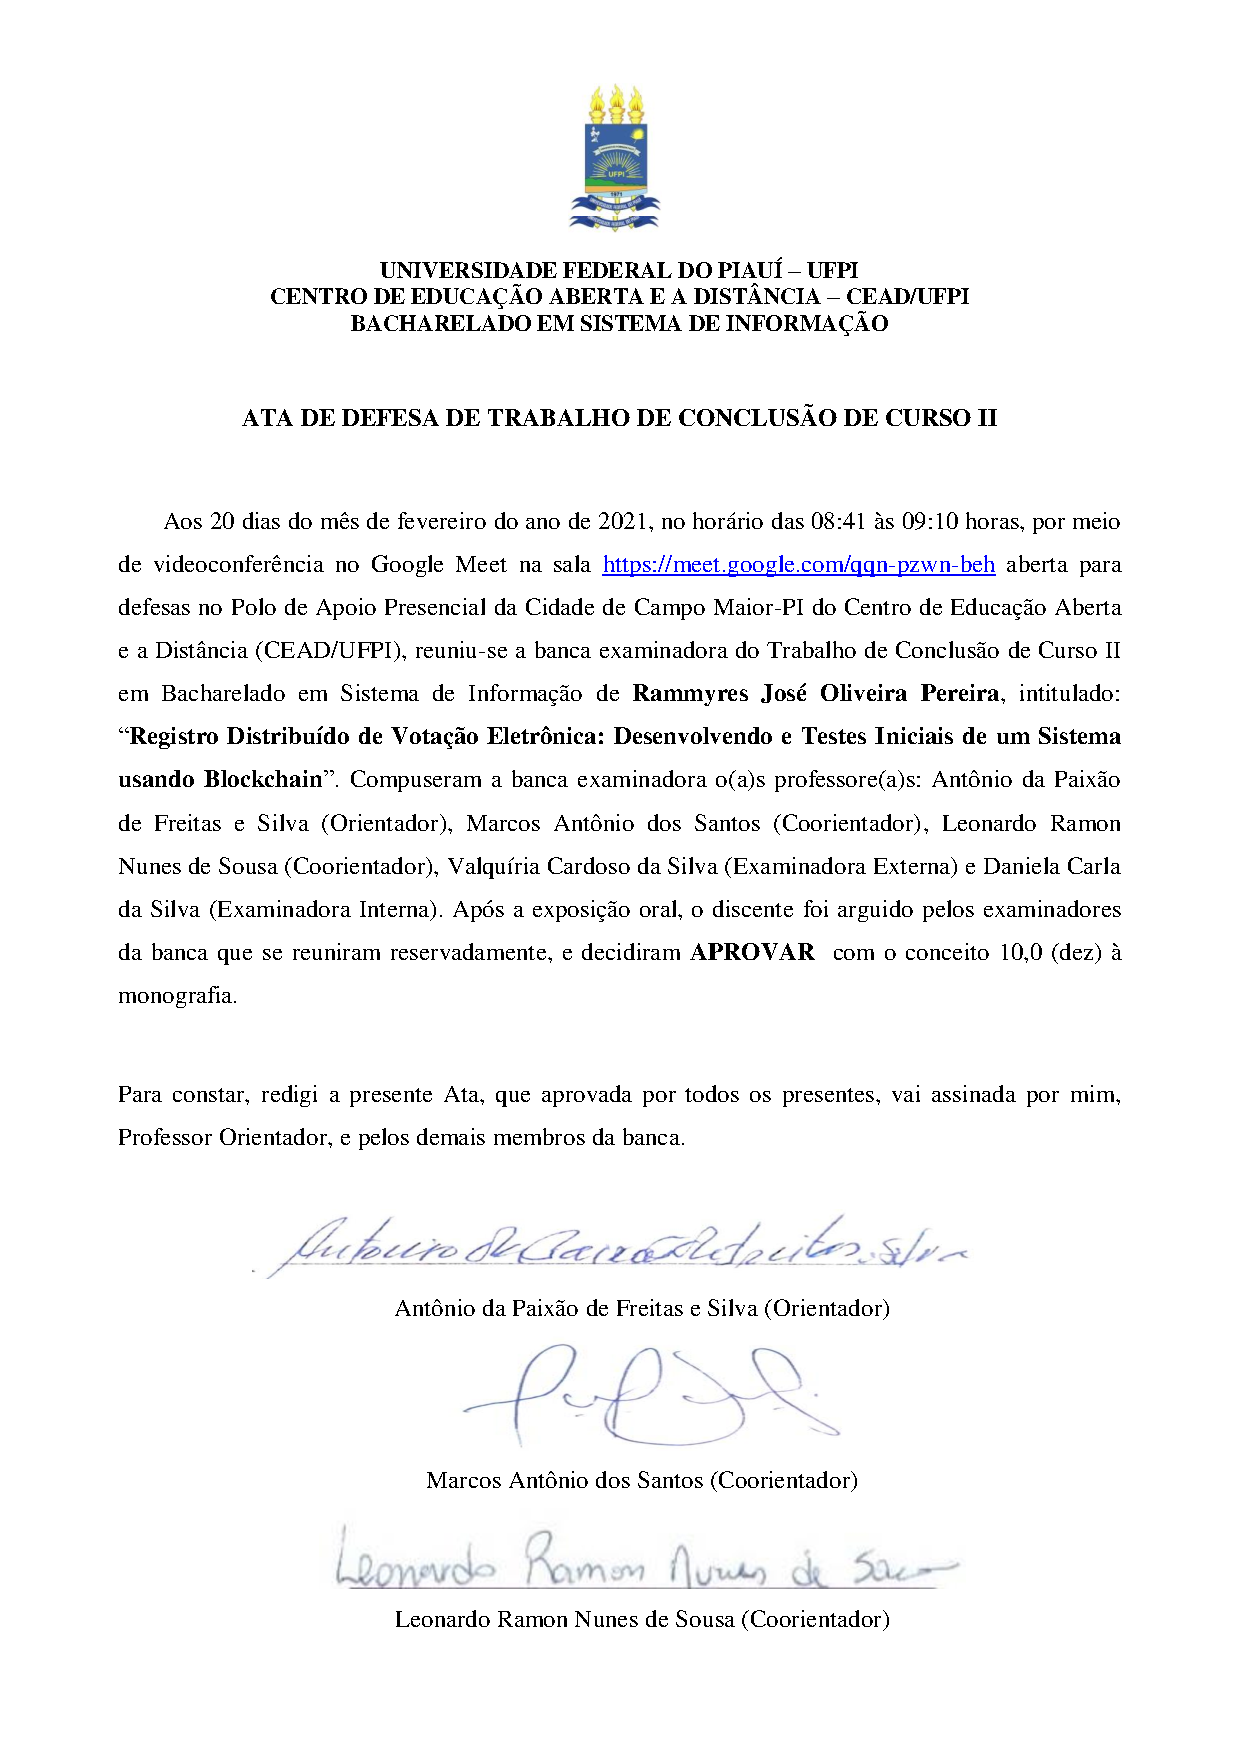
\includepdf[pages=-]{pretextuais/ata.pdf}
% ---
% NOTA DA ABNT NBR 15287:2011, p. 4:
%  ``Se exigido pela entidade, apresentar os dados curriculares do autor em
%     folha ou página distinta após a folha de rosto.''
% ---

% ---
% inserir lista de ilustrações
% ---
%\pdfbookmark[0]{\listfigurename}{lof}
%\listoffigures*
\cleardoublepage
% ---

% ---
% inserir lista de tabelas
% ---
%\pdfbookmark[0]{\listtablename}{lot}
%\listoftables*
\listoffigures*
\cleardoublepage
% ---

% ---
% inserir lista de abreviaturas e siglas
% Edite o arquivo siglas.tex na pasta pretextuais
% ---

\begin{siglas}
  \item[BCS] Blockchain-based crowdsourced systems
  \item[BEV] Blockchain Enabled Voting
  \item[DoS] Denial of Service
  \item[ECDSA] Elliptic Curve Digital Signature Algorithm
  \item[G2B] Government to Business
  \item[G2C] Government to Citizen
  \item[G2G] Government to Government
  \item[JSON] JavaScript Object Notation
  \item[P2P] Peer to Peer
  \item[QR Code] Quick Response Code
  \item[SBSeg] Simpósio Brasileiro em Segurança da Informação e de Sistemas Computacionais
  \item[SBC] Single Board Computer
  \item[UTXO] Unspent Transactions Output
  
\end{siglas}
% ---

% ---
% inserir lista de símbolos
% ---
%\begin{simbolos}
%  \item[$ \Gamma $] Letra grega Gama
%  \item[$ \Lambda $] Lambda
%  \item[$ \zeta $] Letra grega minúscula zeta
%  \item[$ \in $] Pertence
%\end{simbolos}
% ---

% ---
% inserir o sumario
% ---
\pdfbookmark[0]{\contentsname}{toc}
\tableofcontents*
\cleardoublepage
% ---

% ----------------------------------------------------------
% ELEMENTOS TEXTUAIS
% ----------------------------------------------------------
\textual
% ----------------------------------------------------------
% Introdução
% ----------------------------------------------------------
\begin{resumo}
	%Resumo
	\vspace{\onelineskip}
	\noindent
	O objetivo deste trabalho é discutir as tecnologias de votação eletrônica, além de apresentar uma nova alternativa, baseada na tecnologia blockchain, o Registro Distribuído de Votação Eletrônica, bem como discutir seus resultados. Historicamente votar é parte do cotidiano das democracias e com o crescimento delas, organizar o processo de votação e apurar os resultados se tornou cada vez mais desafiador. Por causa disso mecanismos eletrônicos e automáticos para apuração eleitoral se tornaram comuns. O Brasil adotou seu sistema de votação eletrônico na década de 90, entretanto o mesmo tem sido criticado por falhas e falta de transparência. Em 2008 a tecnologia blockchain foi exposta ao mundo, permitindo sistemas transparentes, mas que preservam a privacidade, despertando a atenção de especialistas, que tem se debruçado para criar um sistema de votação baseado em blockchain. 
	Para atender propósito o RDVE será desenvolvido e testado através de eleições simuladas e coleta dos produtos das votações. Como resultado pretendemos avaliar o \textit{software} proposto e analisar sua adequação para atendimento aos quesitos de confidencialidade, confiabilidade e auditabilidade.
	\par\textbf{Palavras-chave}: eleição, votação, eletrônica, digital, blockchain, registro. 
\end{resumo}



\begin{resumo}[Abstract]
\begin{otherlanguage*}{english}  
	\vspace{\onelineskip}
	\noindent
		This paper aims to discuss the voting technologies and propose a BEV alternative, the RDVE (\textit{Registro Distribuido de Votação Eletrônica}), as solution to, at least, some of the issues we discuss here, and analyze its results. Voting is part of our daily life throughout the history of all democracies, and following their growth, the difficulties in the voting processes and tallying  grew in size and complexity. Becausue of this, electronic and automated schemas for ballot processing and counting became commonplace. Brazil adopted its Direct-Recording Electronic Voting Scheme in the 1990s, but, due to failures poited by experts and lack of transparency it has been heavily criticized. In 2008 the blockchain technology was introduced, enabling transparent, yet private, systems, drawing attention from many in industries like finance and e-Government, which in turn has been working towards a secure eletronic voting system. 
		As result we intend to assess the RDVE as solution, specialy aiming its requisites: confidenciality, trustworthiness and auditability. 
		\par\textbf{Keywords}: ballot, blockchain, elections, electronic, tallying, voting.
\end{otherlanguage*}
\end{resumo}
\chapter{Introdução}
Votar é um princípio básico das democracias, das antigas até as modernas e tem sido associado a capacidade popular de tomar decisões e governarem as si próprias. Registros de sistemas de votação datam desde o século VI a.c. \cite{BLACKWELL2003}, quando foi introduzido o modelo ateniense de democracia. Os gregos votavam através dos \textit{ostracon}, fragmentos de cerâmica que retinham, por exemplo, o nome dos cidadãos da \textit{\Gls{polis}} que poderiam ser banidos (ostracismo).  

Ao longo da história o modelo ateniense foi incorporado por outras culturas, como a romana, que adaptaram o conceito de votação através das \textit{leges tabellariae} (\textit{garbinia}, \textit{cassia}, \textit{papiria} e \textit{caelia}) nas decisões populares nos \textit{\gls{comitia}} e eleições de magistrados durante o século II a.c. \cite{Yakobson1995} e avançou até as democracias modernas, que incorporaram conceitos de segredo e privacidade, principalmente através do chamado Voto Australiano \cite{Newman2003} ainda no século XIX.  

O aumento do número de votantes, no entanto, passou a tornar-se um problema. Para exemplificar, o número de votantes nos Estados Unidos em eleições presidenciais subiu de menos de 75.000 em 1800 \cite{VoteArchive2015} para mais quase 136.000.000 em 2016 \cite{VoteArchive2016}. Essa evolução no ínterim exigiu mudanças de estratégias, já que o sistema de contagem voto a voto mostrou-se ineficiente na contagem de tal volume de votos \cite{BATTAGLINI2007}. 

Ainda durante o século XIX as primeiras tentativas de criação de meios automatizados de votação e contagem foram criados, como a “Máquina de Votar Elétrica” de \citeonline{wood_1898}. Durante o século XX muitas tentativas foram abordadas, com o virtual monopólio dos modelos de votação do AVM Corporation nos anos 60 a 80 como destaque \cite{Jones2012}. O Brasil começou a ponderar a utilização de modelos eletrônicos a partir da década de 80 \cite{Brasil2014}, passando a implantar o atual modelo durante a década de 90.  

O modelo adotado por aqui, no entanto, não se livrou de críticas. Durante a primeira e segunda décadas dos anos 2000 problemas como violação do sigilo do voto e execução de código arbitrário puderam ser detectados nas urnas eletrônicas \cite{VandeGraaf2017}, tornando-se alvo de críticas de especialistas \cite{Aranha2018} e de discussões populares \cite{Payao2018}.  

Ao mesmo tempo uma revolução começou a se desenhar com base numa nova maneira de representar dados transacionais. \cite{Nakamoto2008} publicou um artigo descrevendo o que passou a se chamar \textit{blockchain}, uma cadeia crescente de blocos de dados, encadeados entre si através de \textit{\glspl{hash1}} (o bloco atual sempre possuí o \textit{\gls{hash1}} do último bloco). Internamente os blocos são formados por listas de dados, que por sua vez estão conectados entre si através de uma árvore de \textit{\glspl{hash1}}. Todos os nós da rede recebem as transações dela e criam seus próprios blocos e cadeias de dados, impedindo assim a inclusão de dados espúrios; ao manter evidências em diversos computadores diferentes, impede-se que uma transação existente em apenas um nó, ou numa minoria deles, seja considerada válida. 

Isso trouxe ao cenário mundial a ideia de introduzir essa tecnologia para resolução de diversos problemas, como cadeia de propriedade de imóveis e automóveis, transações financeiras, etc. Algumas abordagens para solução serão tratadas ao longo deste trabalho.  

A proposta deste trabalho é discutir essas abordagens, um breve histórico, além de introduzir uma nova proposta, o Registro Distribuído de Votação Eletrônica (RDVE), que tenta permitir a coleta e processamento de votos utilizando registro distribuído em blockchain, bem como discutir sua viabilidade sob aspectos como confiabilidade, confidencialidade e auditabilidade. 
\chapter{Justificativa}
Desprende-se da análise da legislação vigente em relação as Eleições no Brasil a necessidade da manutenção de dois conceitos aparentemente antagônicos entre si: privacidade e publicidade; enquanto é preponderante para manutenção da liberdade de escolha do eleitor, é necessário que o eleitor seja identificado através de dados públicos e a divulgação irrestrita dos resultados das votações. 

A utilização do atual protocolo eleitoral, muito embora preveja mecanismos para garantir que o voto não será associado a seu emissor e haja ampla divulgação dos resultados das votações, a ausência de transparência em várias das etapa não deixa claro como essas proteções são executadas, não parecendo que sejam suficientes para atender aos critérios acima. Os \textit{softwares} e produtos de votação são sigilosos e não há como analisá-los. 

Tecnologias emergentes, como as apresentadas neste trabalho, entretanto são fortemente amparadas em privacidade e publicidade simultâneas. Os protocolos utilizados habitualmente enfocam na manutenção do segredo das identidades das partes que realizam as transações, entretanto todos os registros dessas transações são públicos e acessíveis a todos os usuários da rede, inclusive para os que não fizeram parte delas. A publicidade é tão relevante, que só quando a maioria dos nós da rede podem ter acesso e validar os dados de certa transação é que ela se torna válida, preceito conhecido como consenso, não podendo mais ser revertida. 

Assim sendo nos parece que a utilização dessas tecnologias, com as adaptações necessárias ao atendimento de certas questões legais, é uma alternativa viável para criação de um sistema eleitoral que agregue as características essenciais aqui discutidas. 
\chapter{Problematização}
Questões relacionadas à segurança e privacidade do modelo de votação brasileiro, especialmente a Urna Eletrônica Brasileira, tem sido recorrentes. Em seu livro O Mito da Urna o professor da UFMG, Dr. Jeroen Van de \citeonline{VandeGraaf2017}, explora diversas falhas no nosso modelo de urna eletrônica. Falhas atribuídas a possibilidade de violação de privacidade, violação da integridade dos votos ou recuperação da ordem de votação são discutidas extensivamente no trabalho.  

O professor Dr. Van de Graaf também cita trabalhos do Dr. Diego Aranha, que dedicou atenção especial a falhas contidas na urna eletrônica brasileira, como seu artigo apresentado no SBSeg \cite{Aranha2018}, em que detalha a possibilidade de execução de código arbitrário na urna e seu relatório produzido com base na análise direta do software da urna, “Vulnerabilidades no \textit{software} da urna eletrônica brasileira” \cite{AranhaKMS14}, há menção de erros preocupantes, como a possibilidade de recuperação da ordem dos votantes, implicando em violação de sigilo de voto, além de demonstração de que o processo de cifragem é inadequado e o algoritmo obsoleto. 

Diversas são as críticas traçadas pelos especialistas citados, e muitas são replicadas pelo público geral,  que se foca especialmente na falta de transparência do processo e ausência de auditoria pública. 

O que se questiona neste trabalho é a possibilidade de utilização das tecnologias discutidas, especialmente o Registro Distribuído, para conseguir sanar os problemas levantados, especialmente a ausência de transparência e os questionamentos quanto a privacidade do voto.  
\chapter{Hipotese}
Qual a efetividade do uso de tecnologias emergentes para criação de um protocolo de votação eletrônico descentralizado, que atenda aos prerrequisitos de confidencialidade, confiabilidade e auditabilidade?
\chapter{Objetivos}
\section{Objetivo Geral}
O objetivo deste trabalho é, após analise da literatura existente utilizar \textit{blockchain} para criar um protocolo para votação distribuído, conforme premissas estabelecidas na hipótese.

\section{Objetivos Específicos}
A fim de atingir este objetivo geral, os seguintes objetivos serão seguidos:

\begin{itemize}
	\item Desenhar o protocolo para comunicação entre os nós;
	\item Implementar uma prova-de-conceito em python; e
	\item Efetuar testes públicos para coleta de dados da prova-de-conceito quanto a adequação a hipótese.
\end{itemize}



\chapter{Revisão Bibliográfica}
A tecnologia blockchain foi primeiro descrita por \citeonline{Nakamoto2008}, em seu artigo “\textit{Bitcoin: A Peer-to-Peer Electronic Cash System}”, para descrever um sistema de movimentações financeiras eletrônicas. A ideia essencial seria encadear blocos de transações, ligados entre si através do \textit{hash}, já que cada bloco conteria o \textit{hash} do bloco anterior. As transações seriam assíncronas, propagadas através de uma rede Ponto-a-Ponto, em que cada nó processaria e persistiria a transação em sua própria cadeia, mantendo as evidências de cada transação em uma Arvore de \emph{Hashes} \cite{Merkle1988}, também conhecida como \gls{merkle}, impedindo que uma delas possa ser registrada mais de uma vez. As transações não estariam ligadas a contas, mas a pares de chaves assimétricas, tornando-as virtualmente anônimas. Os nós também precisariam de gasto computacional para computar o \textit{\gls{hash1}} de cada bloco \cite{Nakamoto2008}, utilizando um sistema de \textit{\gls{pow}} \cite{gervais2016}, derivado do algoritmo de prevenção de Negação de Serviço Hashcash \cite{back2002}, desestimulando as tentativas de forjar blocos, já que tal custo seria muito elevado.

A estrutura pensada por Nakamoto estaria protegida contra problemas básicos de redes distribuídas, entre eles a Falha Bizantina \cite{Lamport1982}, que descreve como um nó dispersando informações falsas ou falhas, numa rede distribuída em anel, pode influenciar toda a rede. Outro problema potencialmente resolvível pela proposta, neste caso relacionado aos sistemas financeiros eletrônicos, e bastante relevante nesse contexto, é o problema do gasto duplo \cite{Brands}, que permite um usuário utilizar mais de uma vez um \textit{token} representativo de um valor. A tecnologia de encadeamento de blocos passou a ser conhecida como blockchain e as tecnologias baseadas nela são popularmente conhecidas como Registro Distribuído \cite{Sunyaev2020}.  

Essa abordagem despertou interesse de diversas indústrias, especialmente a financeira \cite{Cahill2020}, fazendo com que muitos acadêmicos também se voltassem para o assunto. Várias análises sucederam a publicação e posterior popularização do Bitcoin e das tecnologias que emergiram a partir dele. Questões tão diversas, que vão a simples cópias do produto original (conhecidas como \textit{Altcoins}) \cite{Nguyen2019}, até a aplicação em cadeias de produção e tributação distribuídas \cite{Choi2019} foram descritas na literatura desde então. 

Em consequência dessa popularidade, questões sobre segurança passaram, também, a serem alvo de constante escrutínio. \citeonline{Ma2020} propuseram uma análise detalhada, após pesquisa em diversas plataformas colaborativas baseadas em blockchain, demonstrando impactos da tecnologia em si, em aspectos relevantes tratados neste trabalho, como privacidade e confiabilidade, utilizando exemplos práticos de tecnologias já implementadas, como registros médicos.  

No mesmo sentido se pronunciaram \citeonline{Zhong2020}, quando analisaram superficialmente os chamados \gls{bcs} (\textit{Blockchain-based crowdsourced systems}), focando nos aspectos mais primordiais do Bitcoin e outras \glspl{criptomoeda}, como segurança e privacidade, da mesma forma que \citeonline{Feng2019}, que especificaram as ameaças mais comuns a serviços baseados na tecnologia, como o comprometimento da privacidade e  disponibilidade da rede (ataques \gls{dos1}), além de relatarem como a implementação correta de um registro distribuído pode contribuir para mitigar tais problemas. 

Considerando as características da blockchain, muitos trabalhos continuaram a seguir, \citeonline{VanLier2017} trata de diversos aspectos metafilosóficos do tema, como as possibilidades de integração entre \glspl{scf} e, obviamente seu uso em sistemas de votação, além da votação interna, para aquisição de consenso. Não demorou para que ideias sobre \textit{\gls{egov}} surgissem e abordassem a utilização dessas tecnologias para permitir o registro de eleições, que de forma geral são conhecidos pela sigla BEV (\textit{blockchain enabled voting}).

\citeonline{Onik2019} descreve em seu trabalho \textit{“Privacy-aware blockchain for personal data sharing and tracking”} mecanismos para registro de informações pessoais, mantendo a privacidade e com mecanismos para controle do compartilhamento dessas informações, baseados nas tecnologias discutidas neste trabalho. No mesmo sentido se pronunciaram \citeonline{Warkentin2020}, ao analisarem a “Tríade da CIA” (i.e. confidencialidade, disponibilidade e integridade) aplicada as tecnologias de blockchain, Noções extraídas da análise também levam em conta a impossibilidade de reversão de atos registrados ou negação de sua autoria, o que tornaria a abordagem relevante para sistemas governamentais, como o exemplo citado no trabalho \cite{Warkentin2020}, no estado de Illinois, onde foram testados diversos usos de registros distribuídos em seu governo. 

Diversos usos para \textit{e-Gov} foram propostos recentemente \cite{Olnes2017}, como modelos de registros de veículos, antecedentes criminais, dentre os diversos usos possíveis. \citeonline{Kshetri2018b} vão mais a fundo, destacando que tais sistemas podem prevenir corrupção e fraudes, em decorrência da publicidade preponderante dos registros e sua forçosa imutabilidade. 

\citeonline{Elisa2018}, em seu artigo “\textit{A framework of blockchain-based secure and privacy-preserving E-government system}” delineia de forma bem detalhada mecanismo de funcionamento de sistemas de \textit{e-Government} baseados em registro distribuído, de forma geral, incluindo todos os serviços de \gls{g2g}, \gls{g2c} e \gls{g2b}. 

Historicamente o TSE \cite{Brasil2014} demonstrou interesse em informatizar o sistema de votação Brasileiro desde a década de 80, tomando medidas para informatização das Urnas durante a segunda metade da década de 90. O modelo brasileiro de votação eletrônica atualmente é adotado em todo o território nacional, para todas as eleições majoritárias e proporcionais.    

O impacto da confiança da população em tecnologias como essa já foi explorando, para o uso em sistemas governamentais complexos, como o sistema de votação brasileiro. \citeonline{Moura2017}, apresentaram a percepção negativa dos atuais sistemas eletrônicos de votação, bem como a visão positiva de um sistema baseado em blockchain.  

As ideias, no geral, dão conta que um sistema de votação BEV seria percebido como mais transparente, confiável e auditável, já que seu resultado, o Registro Distribuído, é público e disponibilizado a todos os nós e clientes ligados a rede.  

\citeonline{Curran2018} cita as dificuldades do dito \textit{E-Voting}, que é o termo genérico para votações eletrônicas que não dependam de maquinário específico, e habitualmente propõem a utilização de meios eletrônicos para apuração de votos online, com o uso de aplicativos e \textit{websites}. Potenciais falhas e abertura a fraudes, além das dificuldades de auditar tais sistemas são citados como principais motivos da rejeição da adoção desse modelo.  

Dificuldades para atrair eleitores, especialmente os mais jovens, mais facilmente atraídos por tecnologia e menos por ambientes burocráticos, causando aumentos sucessivos das abstenções, também são dificuldades trazidas as eleições, tanto tradicionais em papel, quanto as utilizado sistemas de votação eletrônico. Entretanto vê a possibilidade de inclusão de sistemas com blockchain para registro e apuração de votos como um meio de desenvolvimento de \textit{apps} e \textit{websites} suficientemente confiáveis para registro de votações eletrônicos.

Dentre os possíveis resultados citados por \citeonline{Curran2018} também constam possibilidades, julgadas por muitos como necessárias, de auditabilidade, tanto individual (i.e., o eleitor é capaz de verificar seu próprio voto) como publica (i.e., é possível a qualquer pessoa auditar a votação como um todo).  

\citeonline{Abuidris2019} fizeram uma pesquisa sobre uma série de soluções propostas para os conceitos levantados por Curran. Os estudiosos identificaram, pelo menos, seis propostas, dentre elas os sistemas \textit{Follow My Vote}, \textit{Agora} e \textit{Polys}, que tem relativa notoriedade. 

Todos esses sistemas têm, como funções básicas, a persistência dos votos em um Registro Distribuído, entretanto com grande enfoque em soluções que não dependam de pontos de coleta de votos, nem maquinário específico, já que eles serão colhidos através de \textit{apps} ou \textit{websites}. Os autores também fizeram uma análise comparativa a respeito de diversas características das soluções, como auditabilidade, descrita nos trabalhos como “verificabilidade” (tradução livre), tanto individual como pública (descrita como “universal”), e listaram objetivos a serem alcançados em soluções futuras, como um meio de identificar eleitores, sem comprometer o sigilo do voto, tornar as experiências de usuários simples o bastante a fim de tornar o acesso fácil a todos os segmentos da população, mecanismos para garantir a escalabilidade e expansão da base de usuários, além de meios para aprimorar a velocidade para inserção dos votos e do processo de apuração.  

\citeonline{Wang2018}, em seu artigo \textit{Large-scale Election Based On Blockchain}, propuseram a ideia de um sistema de contratos inteligentes, codificados sobre a plataforma de criptomoedas \gls{eth}. A proposta, conforme apresentada utilizaria \gls{homo} e assinatura em anel, a fim de preservar a integridade e anonimato da votação na rede, o que implicaria na preservação da privacidade no sistema; todas as fases, incluindo o registro do eleitor e a apuração dos votos seriam completamente anônimos, o que inviabilizaria um processo de auditoria externa. 

\citeonline{Srivastava2018} apresentaram artigo descrevendo um protocolo de votação usando uma das formas de blockchain, desenvolvido com base numa tecnologia derivada deste, que permite a formação de grafos acíclicos, enfatizando a privacidade.  

As ideias quanto as implementações dos sistemas de votação são diversas, especialmente quando tomamos analogias aos maiores sistemas de uso de registros distribuídos, que são as criptomoedas. 

A ideia mais comum é a de gerar “carteiras” onde cada usuário (eleitor) recebe uma “moeda” e pode “gastá-la” em um voto, como descrito por \citeonline{Kshetri2018a}. Os autores classificam esse ramo de estudo de \textit{Blockchain Enabled Voting}, ou BEV, que possui as aplicações e modelos já levantados anteriormente, entretanto enfocando a tecnologia para diversos tipos de votações, inclusive as que não envolvam cargos eletivos, como plebiscitos e consultas públicas. Uma vantagem, no entanto, enfatizada pelos autores, está na dificuldade ou impossibilidade de criar votos falsos, ou fraudes no próprio registro de votação, o que parece ser um tema comum em todos os trabalhos até aqui descritos. Da mesma forma se posicionam \citeonline{Agbesi2019}, que apresentaram em Copenhagen um protocolo bastante detalhado de votação, também baseado na ideia da criação de carteiras e distribuição de moedas previamente a votação.  

Temores de fraudes costumam ser ideias centrais da literatura do tema, como mencionado por \citeonline{Zhang2020}. Um dos principais propósitos de sistemas com registro distribuído de votos seria dificultar ao máximo o uso de mecanismos fraudulentos de votação e registro, quer pela exploração de falhas nos \textit{software} ou pelo uso de mecanismos sociais. Uma das ideia ventiladas seria a concessão de "recompensas" para bons eleitores e registradores de votos, bem como penalidades para os suspeitos de fraudes. Do mesmo modo se pronunciam \citeonline{Zhou2020}, numa análise preliminar sobre os principais mecanismos de privacidade nos sistemas de votação eletrônica disponíveis, a saber: assinaturas cegas, em anel ou por delegação.  

\citeonline{Li2020} propuseram a combinação das tecnologias aqui descritas com a \gls{iot}, permitindo sistemas de contagem automática de votação, com \textit{software} executando em maquinário de baixo custo, tornando a captura e processamento de votos amplamente acessível e uma votação de grande porte barata; tal posição foi compartilhada em proposta de \citeonline{Krishnamurthy2020}, que também detalharam diversos mecanismos de segurança associados a mecanismos de votação e contagem. 

A performance de sistemas blockchain para votação também foi abordado em trabalhos anteriores. Os tempos de entrada e apuração podem ser fatores preponderantes, entretanto quando ajustados apropriadamente podem propiciar velocidade suficiente para que seu uso possa ser levado em consideração para grandes projetos de BEV \cite{Khan2020}.  

Conforme se conclui, a utilização de BEV foi bastante escrutinada nos últimos anos, em vários aspectos e sob diversos prismas. A concordância das diversas publicações do uso de blockchain para \textit{\gls{egovs}} e, especialmente para votação, parece estar se formando. Sistemas informatizados inovadores, baseados em \textit{hardware} de baixo custo e \textit{software} alicerçado em tecnologias emergentes podem ser capazes de produzir sistemas de votação com publicidade e confidencialidade, termos aparentemente antagônicos, mas necessários a um sistema que atenda a proposta deste trabalho. A combinação dos elementos apresentados podem apresentar respostas a questionamentos históricos da votação eletrônica, como a possibilidade de auditoria e manutenção da privacidade dos votantes, tornando o registro distribuído uma alternativa aparentemente viável e eficaz.  
\chapter{Metodologia}

O método escolhido para atingimento dos objetivos aqui descritos é a experimentação, através da implementação de uma prova de conceito baseado no modelo proposto e a realização de votações simuladas, utilizando-se esse \textit{software}, procedendo a coleta do produto da execução para apuração e análise utilizando-se uma abordagem qualitativa. Este trabalho abordará sistemicamente o processo de produção e testes, registrando estes processos e seus resultados.  

A solução será implementada para execução em hardware genérico, com a configuração composta especificamente de uma placa SBC (\textit{\gls{sbc1}}, ou computador de placa única) \gls{rpi}, telas sensíveis ao toque com câmera embutida. Além da plataforma será desenvolvido um aplicativo, para o sistema operacional Android, que permitirá a gestão das identificações dos usuários, através de pares de chaves \gls{ecdsa1}, além de permitir a comunicação com o hardware através de \textit{\glspl{qr1}}.  Os produtos das votações serão colhidos em memória \textit{flash} (pendrives ou cartões de memória) e analisados através de \textit{software} automatizado. Eles também terão seus resultados armazenados de forma pública, para inspeção pelos interessados. Por fim o resultado será processado através de uma rede distribuída \gls{p2p}. 

O \textit{software} de coleta e dos nós da rede distribuída serão criados desenvolvidos em Python, o \textit{app} será desenvolvido em Dart.  

Considerando os aspectos subjetivos levantados neste trabalho, referentes a conceitos como confiabilidade, privacidade, etc., nos parece haver a necessidade de uma posição interpretativa quanto ao conjunto de ações essenciais a conclusão das ações descritas nos objetivos, bem como a análise de seus resultados. A partir daí será necessário explorar as possibilidades de utilização do modelo descrito acima, através de experimentação.

De forma resumida: 
\begin{itemize}   

\item Abordagem: qualitativa; 
\item Posição epistemológica: interpretativa;
\item Método de pesquisa: experimental;
\item Finalidade: exploratória;
\item Técnica de coleta: observação direta; e
\item Técnica de análise: análise de conteúdo.
\end{itemize}
\chapter{Proposta de trabalho}

\textit{Blockchain} se tornou um assunto recorrente nos últimos anos. O assunto tem se tornado relevante, tanto pela adoção massiva em criptomoedas, como pelo recente interesse do sistema financeiro tradicional. Em movimento inédito a China tem testado uma versão digital do Yuan \cite{Carvalho2020}. O interesse chegou também ao Brasil e o Banco Central tem ventilado a possibilidade de um Real Digital, baseado em DLT \cite{Tecmundo2021}.

As tendências de agregar a tecnologia aos sistemas de votação existente também tem ganhado momento. Trabalhos como \citeonline{Patidar2019}, \citeonline{Mpekoa2017}, \citeonline{Ahmed2020}, \citeonline{Bistarelli2019} e \citeonline{Yi2019} tem demonstrado a tendência da comunidade acadêmica quanto ao uso das tecnologias aqui discutidas. O interesse também foi despertado o interesse do TSE \cite{GUSSON}. 

A proposta deste trabalho, a fim de testar hipótese apresentada, seria o desenvolvimento de provas de conceito, com base em um protocolo desenhado para comunicação entre nós e testes públicos, entretanto a abordagem foi dificultada pela pandemia mundial de COVID-19. Assim sendo, a fim de dar prosseguimento a testagem da hipótese, dois aplicativos, detalhados adiante, foram desenvolvidos e testados, a fim de aferir a hipótese deste trabalho. 
\chapter{Resultados}

Considerando a bibliografia explorada, foram detectadas tendências nas pesquisas atuais. Os modelos mais comuns de estruturas utilizadas pelos pesquisadores mundo afora incluíam, principalmentel \textit{apps} para coleta e processamento dos dados da votação. 

A partir da proposta de trabalho foram desenvolvidos dois aplicativos, RDVE Wallet e RDVE Coleta. 

\section{Estrutura básica do projeto}
É preciso, antes de detalhar de forma mais aprofundada os resultados do desenvolvimento, explicar alguns conceitos básicos utilizados em tecnologias de registro distribuído. 

\subsection{Chaves assimétricas}

São pares de chaves utilizados para identificar os usuários em transações computacionais. O par de chaves é composto por uma chave privada, que é capaz de produzir uma assinatura única e identificável, vinculada ao usuário que a gerou. A validação é feita através da utilização de uma chave pública, que é disponibilizada publicamente. Cada par de chaves é único e são vinculados um ao outro de forma que dados assinados por uma chave privada só podem ser validados por sua respectiva chave pública. 

\subsection{Endereço}

O endereço é uma particularidade de sistemas \textit{blockchain}. Trata-se de uma versão reduzida da chave pública do usuário, processada por diversos algoritmos criptográficos de assinatura.

No caso especifico do sistema RDVE a chave pública passa pelos seguintes algoritmos, nesta ordem:

\begin{itemize}
	\item SHA256
	\item SHA256
	\item RIPEMD-160
	\item a representação hexadecimal do sumário RIPEMD-160 recebe o prefixo 'x00'
	\item Os quatro últimos dígitos do sumário SHA256 do item anterior é anexado ao final da \textit{string} formada pelo sumário RIPEMD-160 e o prefixo 'x00'
	\item o resultado da ultima transformação é representado como um numero representado em Base 58 \cite{Nakamoto2019}	
\end{itemize}

\begin{figure}[!h]
	\centering
	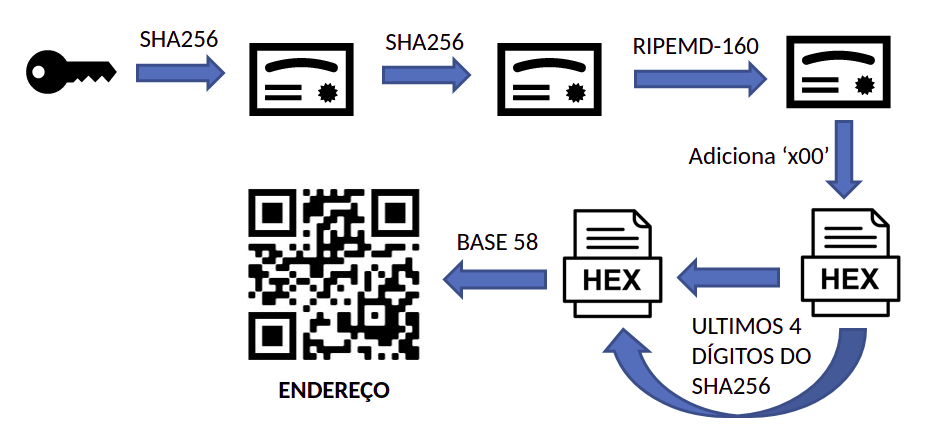
\includegraphics[width=0.9\textwidth]{imagens/fluxo_endereco}
	\caption{Fluxograma de geração do endereço}
	\label{fig:fluxo_endereco}
\end{figure}
%\clearpage

Em protocolos como o Bitcoin a chave pública não é divulgada fora das \textit{wallets}, em decorrência da possibilidade de, no futuro, a utilização do Algoritmo de Shor permita a obtenção da chave privada a partir da chave pública \cite{Mavroeidis2018}. 

Ainda que um computador quântico com \textit{\glspl{qubit}} suficientes para o processamento de um algoritmo de fatoramento de grandes números ainda não esteja no horizonte, a solução utilizada no Bitcoin pode implicar na resistência a tal brecha no futuro e foi adotada neste trabalho. 

\subsection{UTXO (Unspent Transactions Output)}

O Saldo de Transações Não-Gasto (UTXO) é uma lista, composta por todos os endereços registrados na rede, seu saldo atual e uma lista interna contendo todas as transações em que aquele endereço foi parte, seja de entrada ou saída. A lista é produzida a partir do processamento das transações existentes nos blocos, permitindo uma leitura mais simples dos saldos, sem a necessidade de procurar cada uma das transações nos blocos.

\subsection{Assinatura por delegação}

Assim como as chaves, o endereço identifica os usuários em uma rede \textit{blockchain}, mas, no caso especifico deste trabalho, também identifica as urnas, permitindo que os eleitores transfiram seus saldos de votos para elas, permitindo que as urnas assinem as cédulas virtuais de votação no momento da coleta dos votos, desta forma as urnas recebem a delegação dos usuários para assinarem as cédulas, ocultando os dados dos votantes.

\subsection{Bloco Registros}

Os blocos registros são blocos que contém as transações de criação de endereços, funcionando de forma similar a um banco de dados contendo endereços de todos os participantes da rede, incluindo ID dos eleitores, mesários e urnas (gerados a partir do algoritmo UUID4), nomes dos eleitores, apelidos e números dos candidatos. 

\subsection{Cédula}
É a abstração de uma cédula em papel, contendo campos específicos para assinatura (produzida pela urna) e o endereço de destino, referente ao candidato votado.

\subsection{Requisição de votação}
É a transação pela qual o eleitor transfere para urna seu saldo no sistema, permitindo que a mesma requeira uma cédula para que o eleitor registre seu voto. A requisição de votação também funciona como prova de comparecimento do usuário. 

\subsection{Bloco Produtos de Votação}

É o resultado da votação, produzido pelas urnas e contém as transações de transferências dos saldos dos eleitores para as urnas (uma unidade por vez) e das urnas para os candidatos, conforme votação.

\section{RDVE Wallet}

O primeiro aplicativo, desenvolvido em linguagem \textit{Dart} utilizando-se o \textit{framework Flutter} foi o \textit{\gls{wallet}} RDVE Wallet\footnote{Código fonte disponível em \url{https://github.com/rammyres/rdve_wallet}}, que permite a identificação do usuário no sistema. 

O aplicativo possui um módulo principal, capaz de gerar e gerenciar chaves criptográficas que identificam o usuário. 

\begin{figure}[!h]
	\centering
	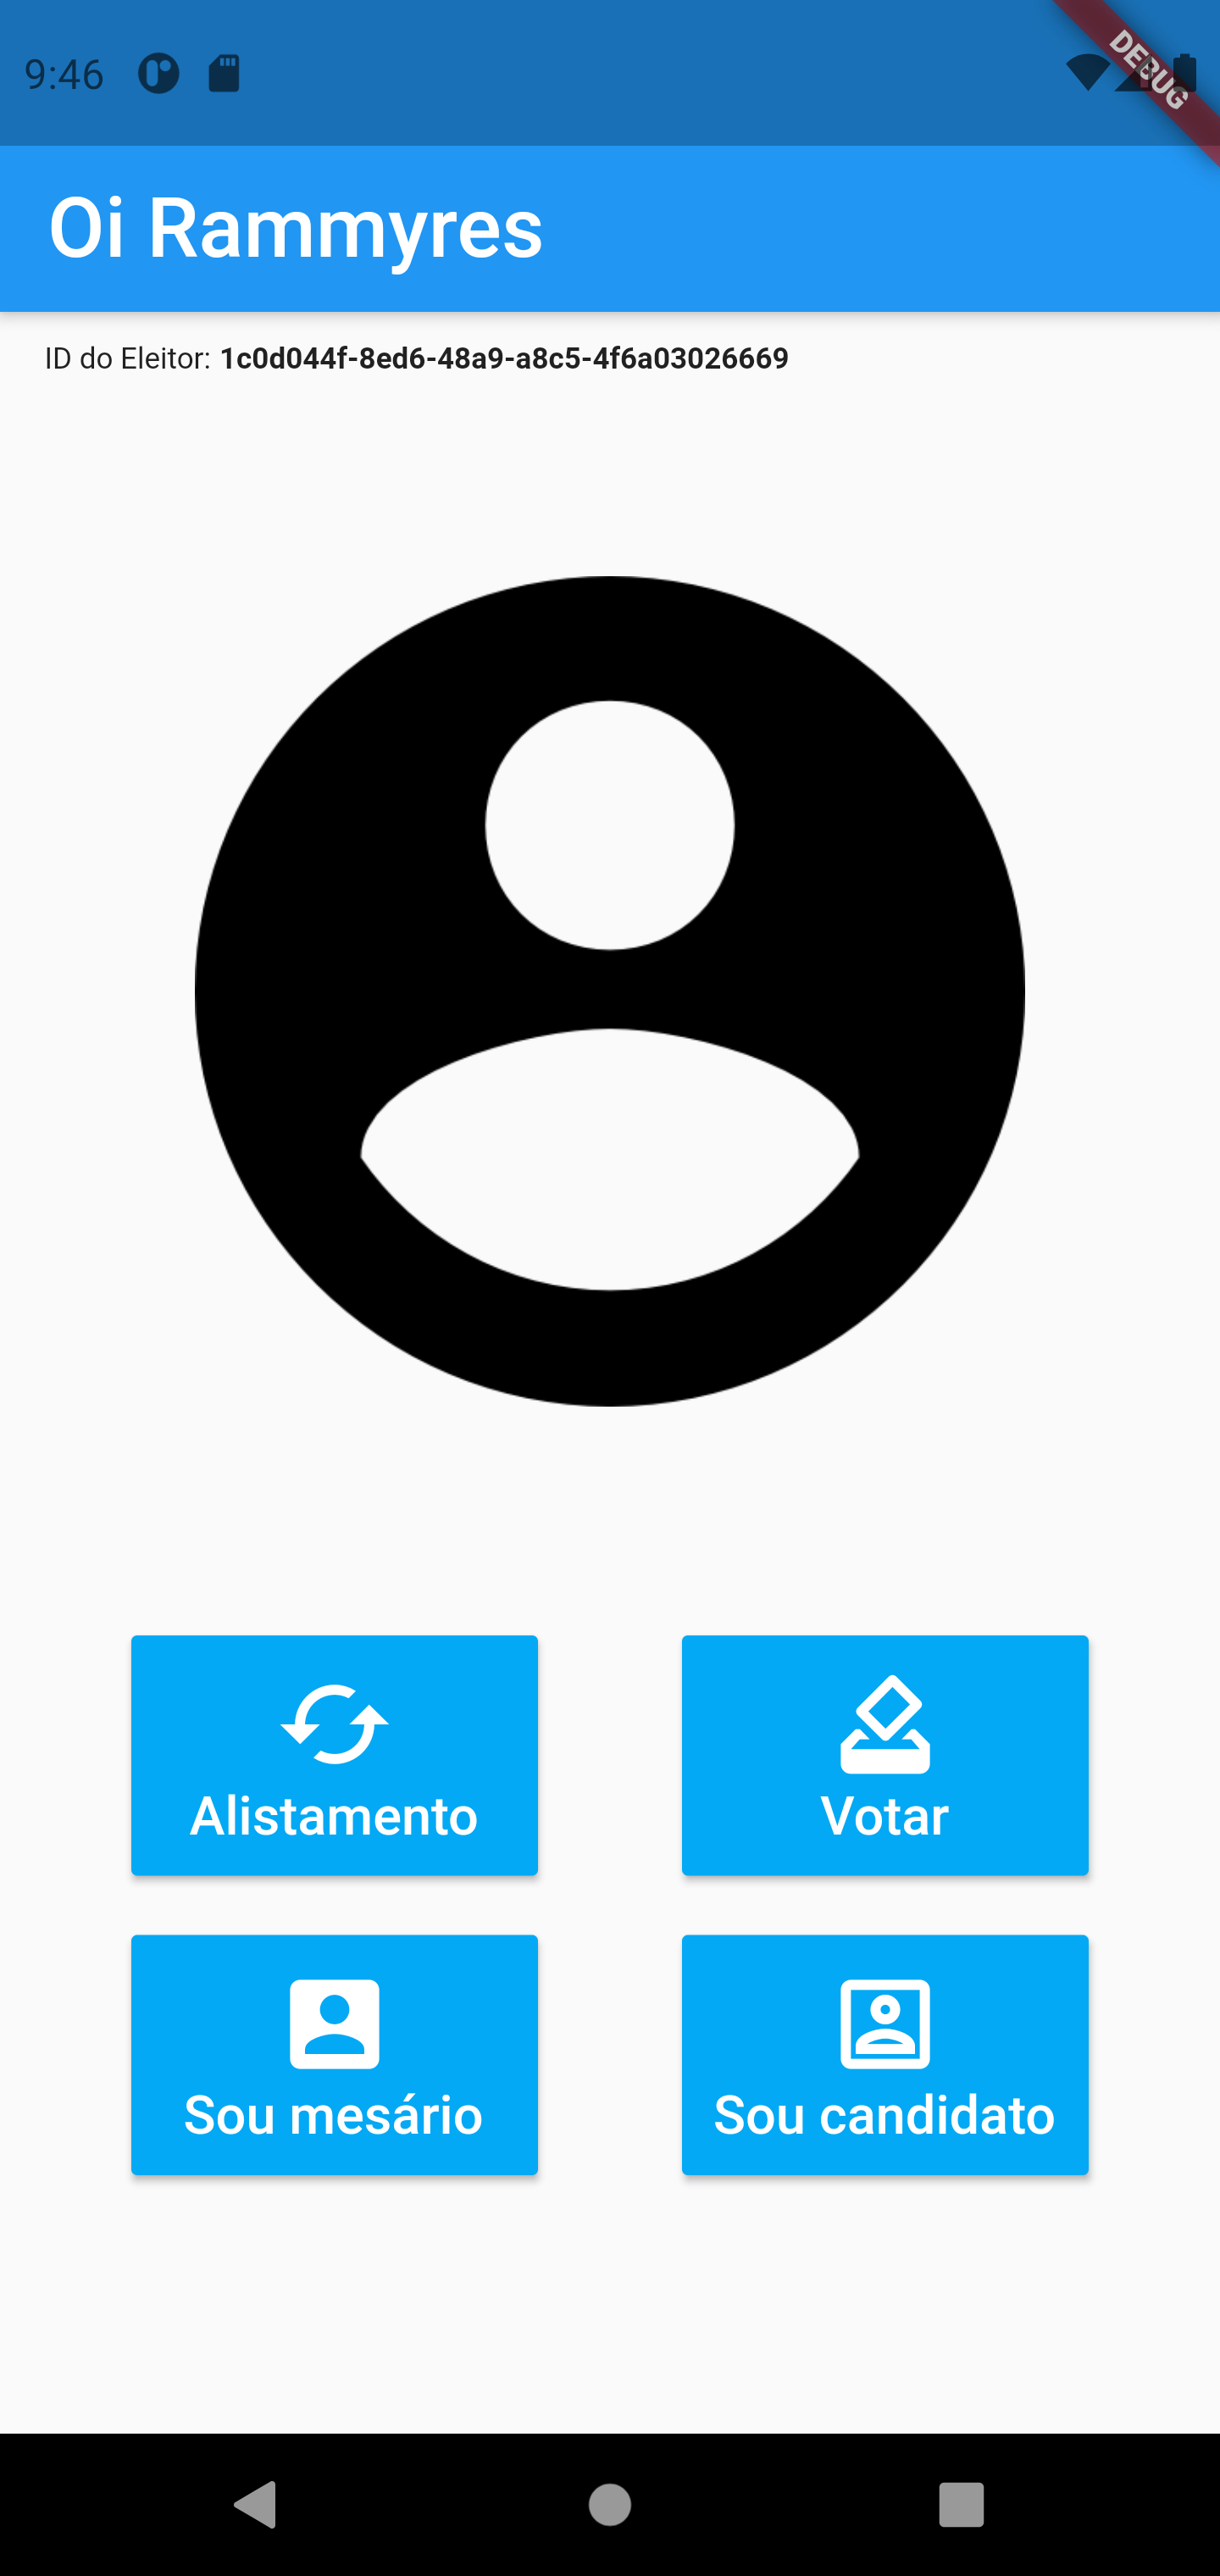
\includegraphics[width=0.5\textwidth]{imagens/wallet1}
	\caption{Módulo principal do RDVE Wallet}
	\label{fig:wallet1}
\end{figure}
\clearpage


A ID do eleitor identifica o mesmo dentro de todo o sistema, inclusive quado o mesmo se candidatar a cargo eletivo. Uma vez registrado no sistema o usuário pode requerer seu alistamento como eleitor, utilizado o módulo alistamento do aplicativo RDVE Coleta. Os dados são codificados como um objeto \gls{json}, contendo os dados necessários ao registro do usuário e apresentados como um \gls{qr1} que pode ser lido por outros dispositivos de modo \textit{offline}. 

\begin{figure}[!htb]
	\centering
	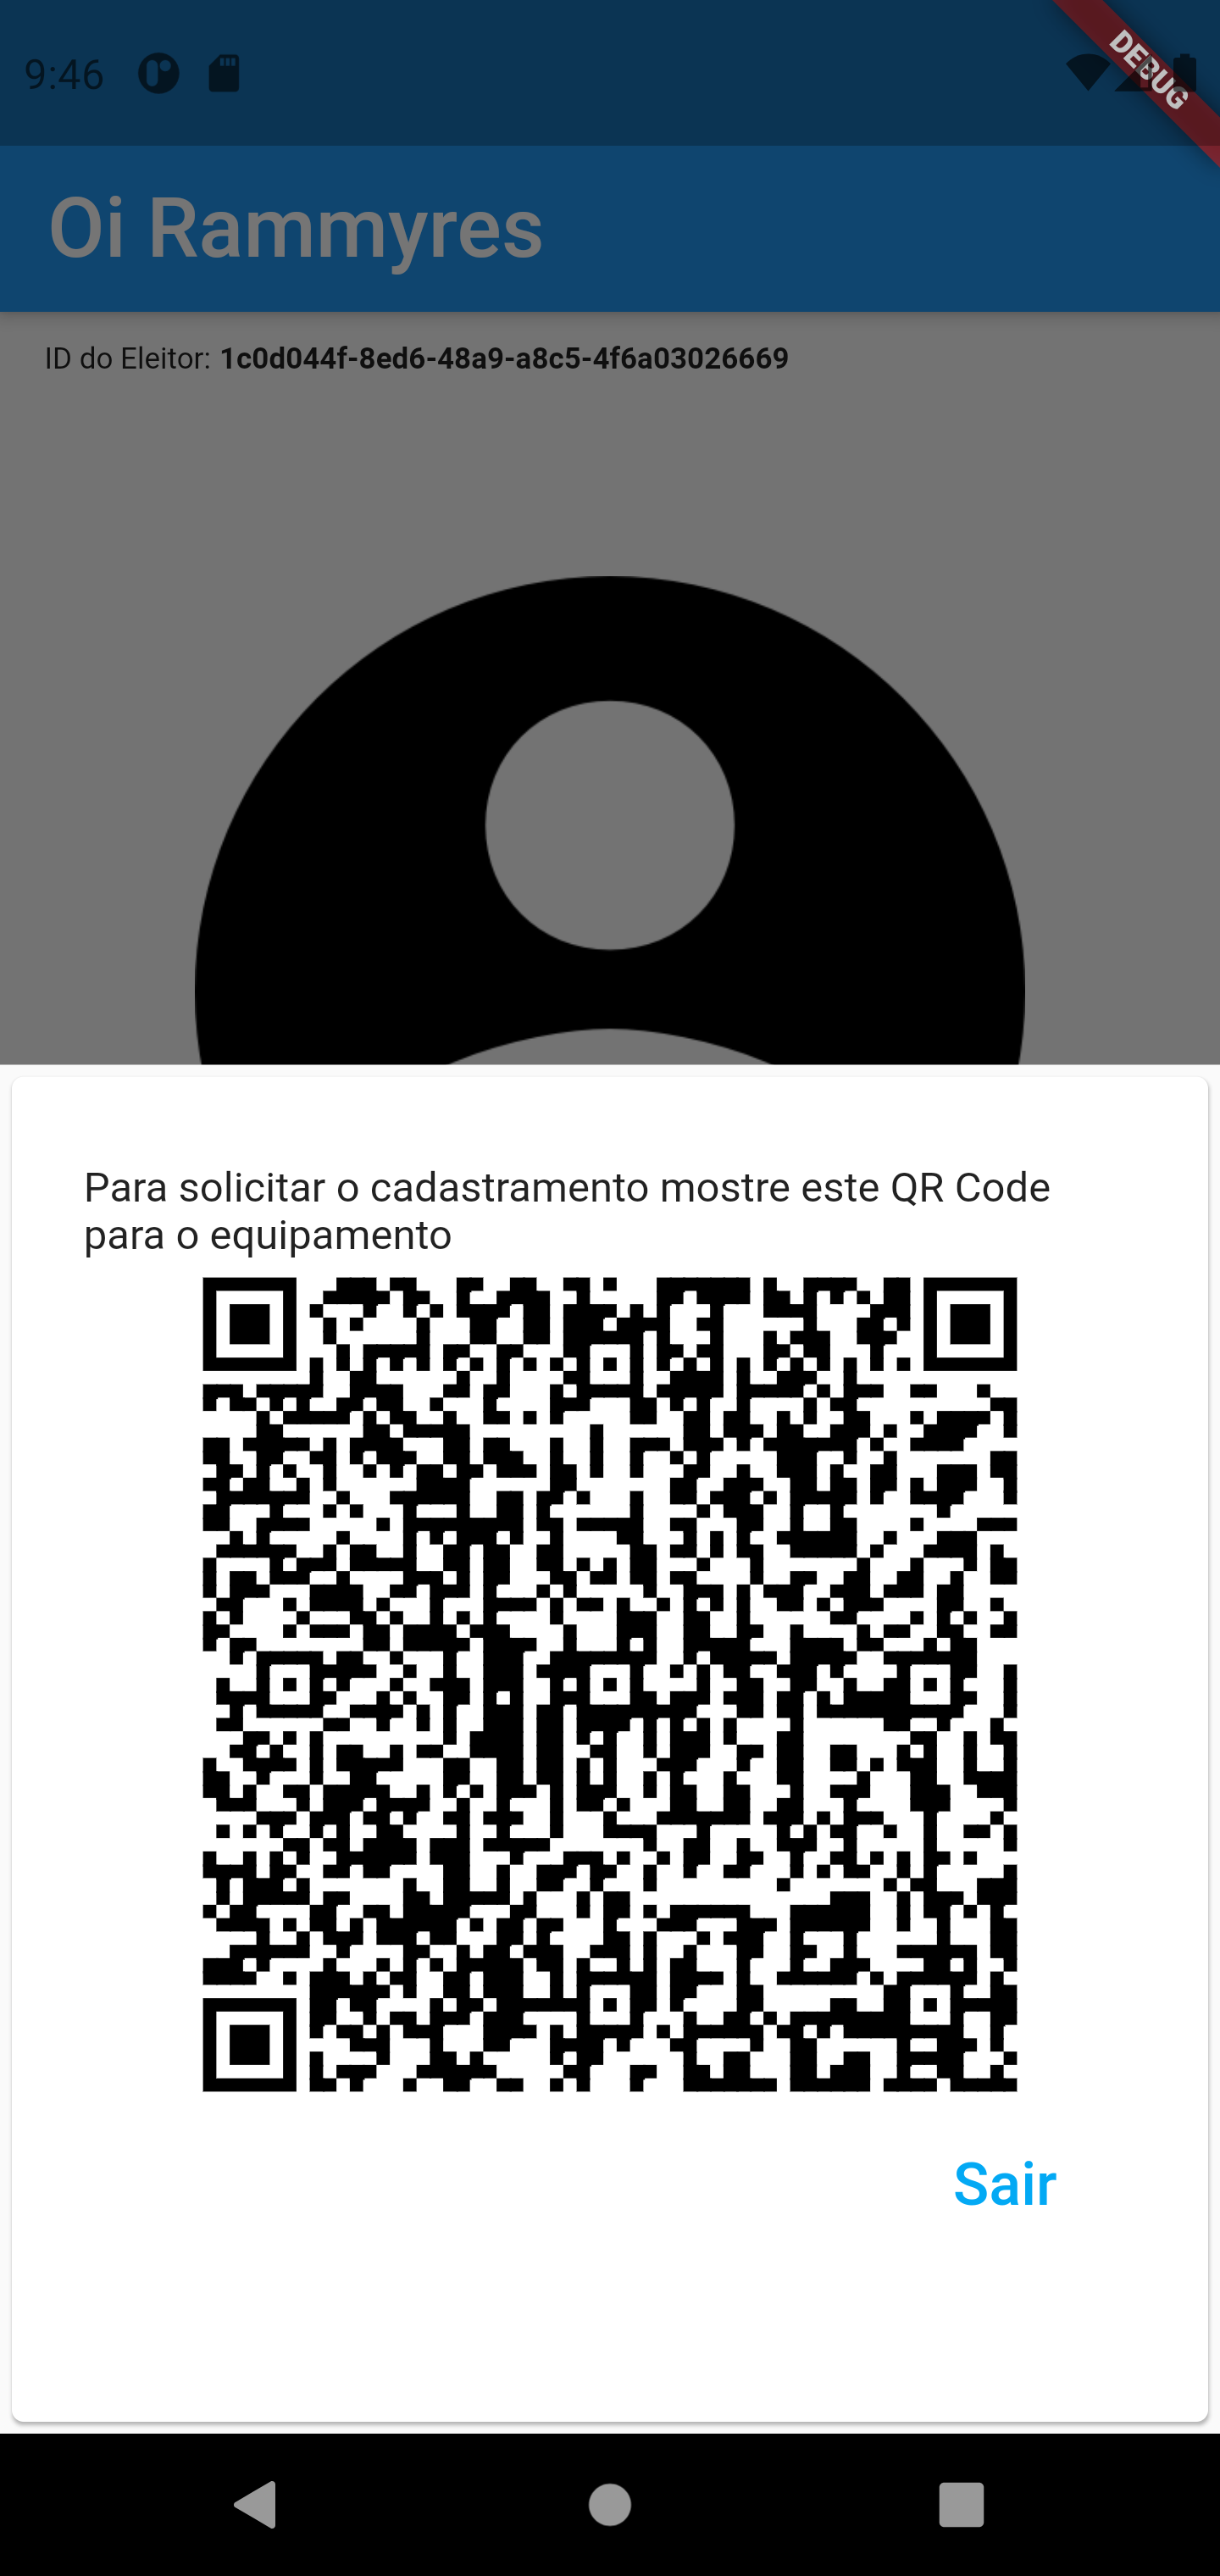
\includegraphics[width=0.5\textwidth]{imagens/wallet2}
	\caption{Módulo de alistamento}
	\label{fig:wallet2}
\end{figure}

De forma similar, existem módulos para registro como operador de urna (mesário) e candidatura. No primeiro caso não há geração de novas chaves criptográficas. 

\begin{figure}[!htb]
\centering
\begin{minipage}{0.47\textwidth}%	
	\centering
	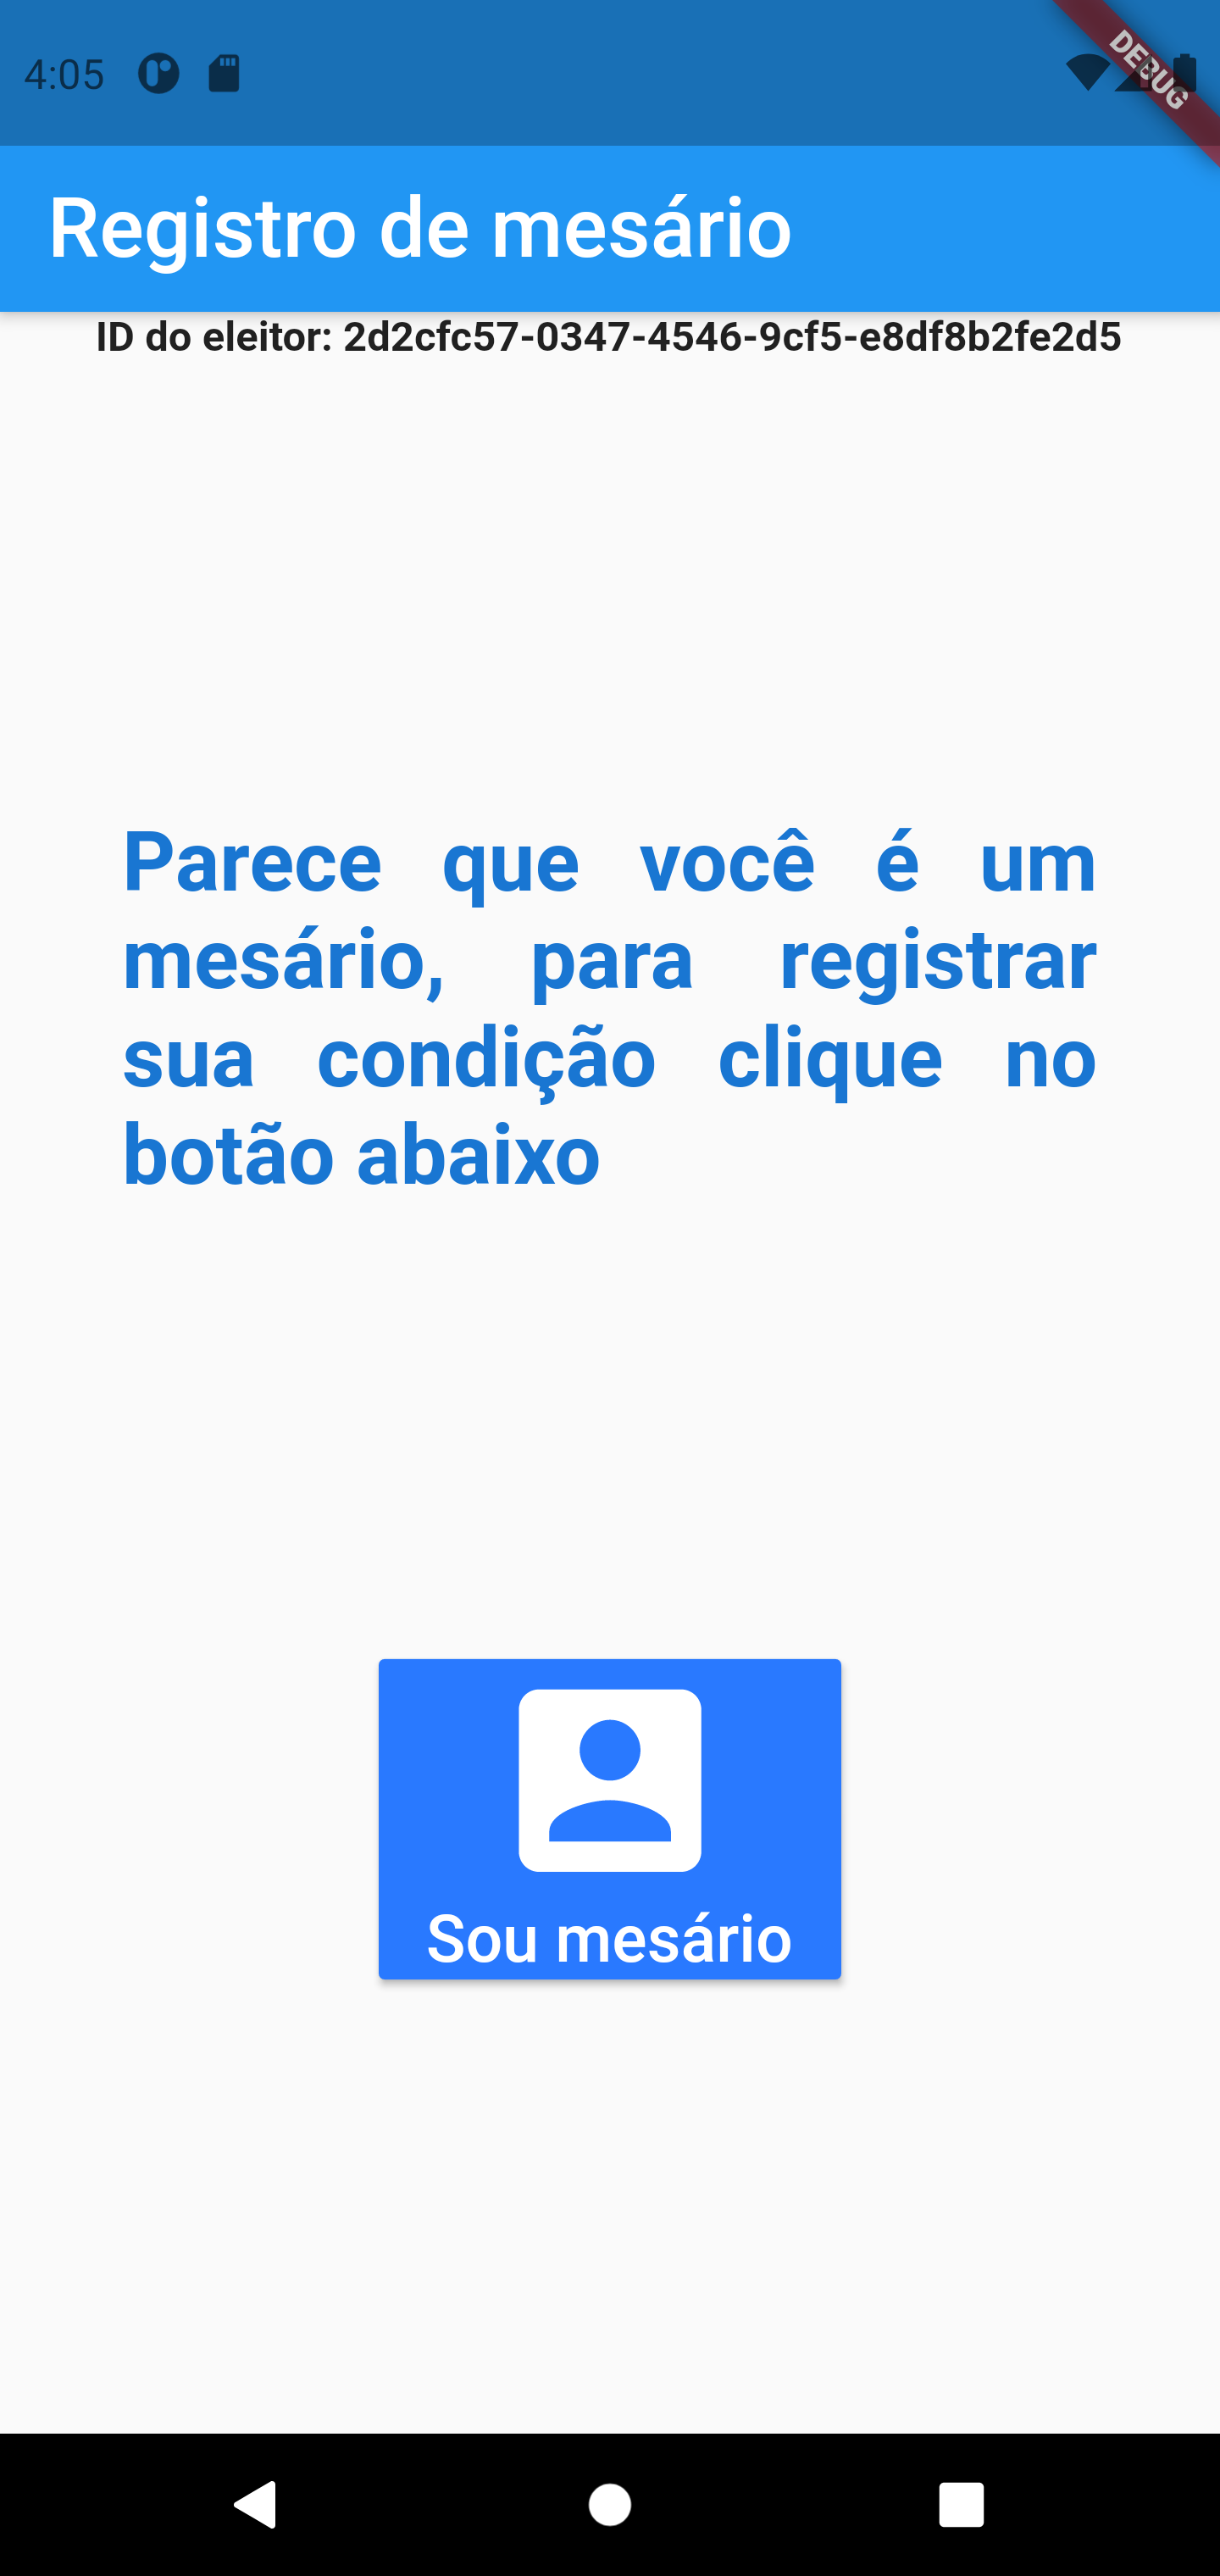
\includegraphics[width=.9\textwidth]{imagens/wallet_mesario}
	\caption{Módulo de registro do operador de urna}
	\label{fig:wallet_mesario}
\end{minipage}
\hfill
\begin{minipage}{0.47\textwidth}%
	\centering
	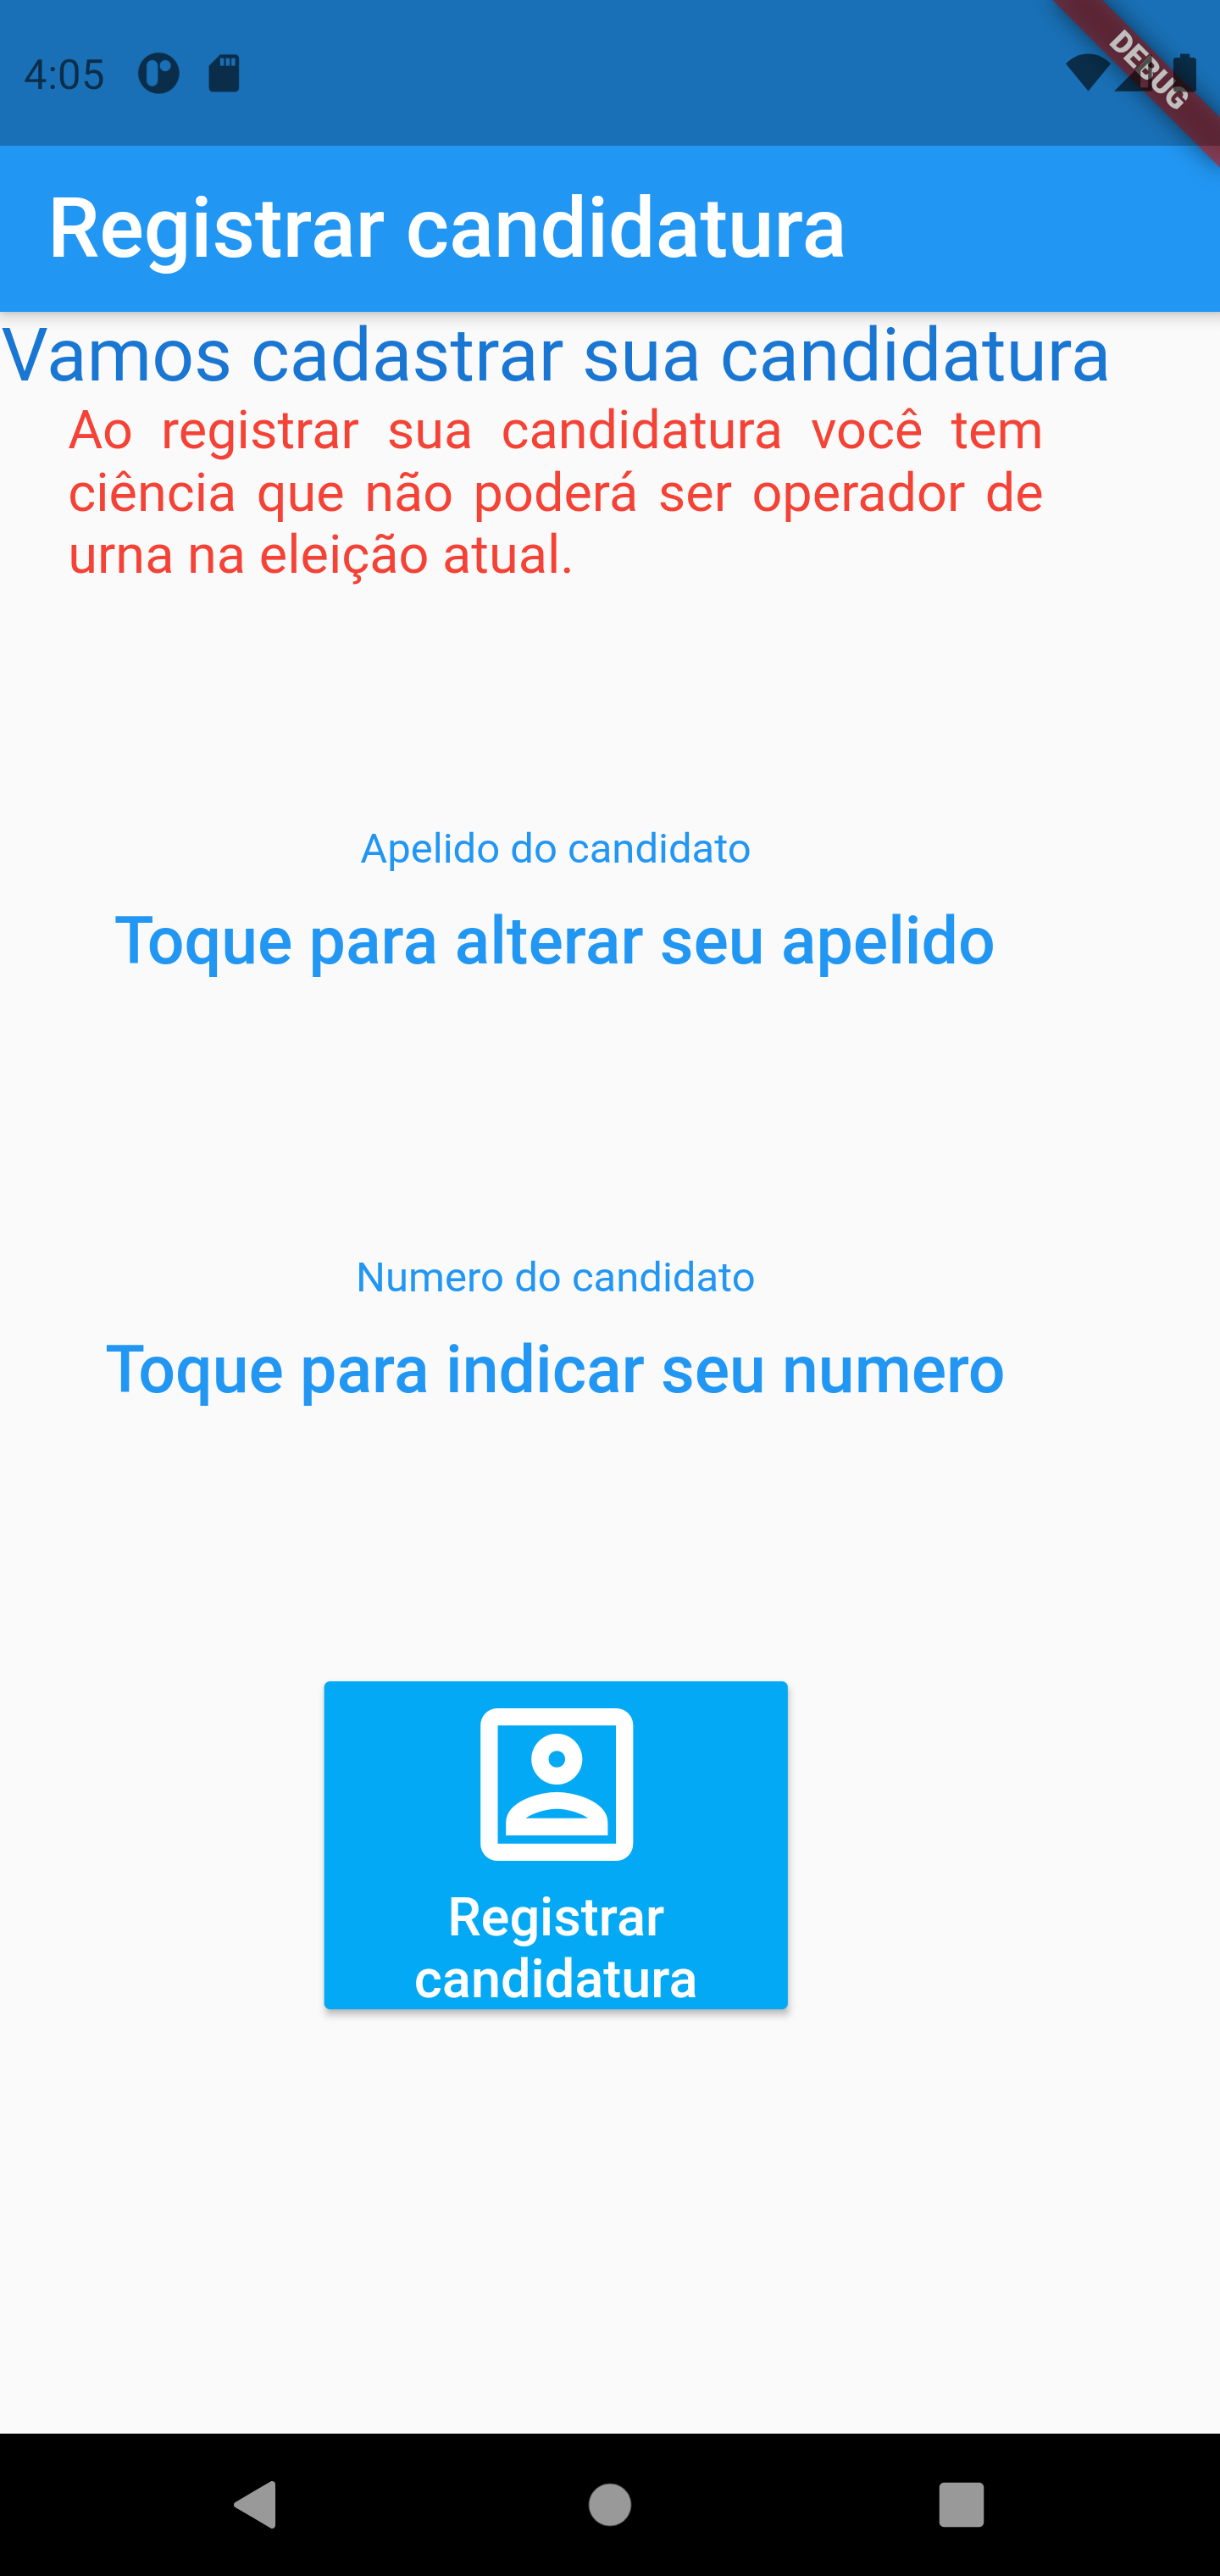
\includegraphics[width=.9\textwidth]{imagens/wallet_candidatura}
	\caption{Módulo de registro de candidatura}
	\label{fig:wallet_candidato}
\end{minipage}
\end{figure}
\clearpage

A comunicação com o sistema de coleta utiliza o mesmo princípio, gerando \glspl{qr1} contendo os dados necessários ao cadastramento de operadores e candidatos. 

Por fim o módulo de operação de urna permite que o mesário libere o alistamento eleitoral, o registro de candidatura e o voto. 

\begin{figure}[!htb]
	\centering
	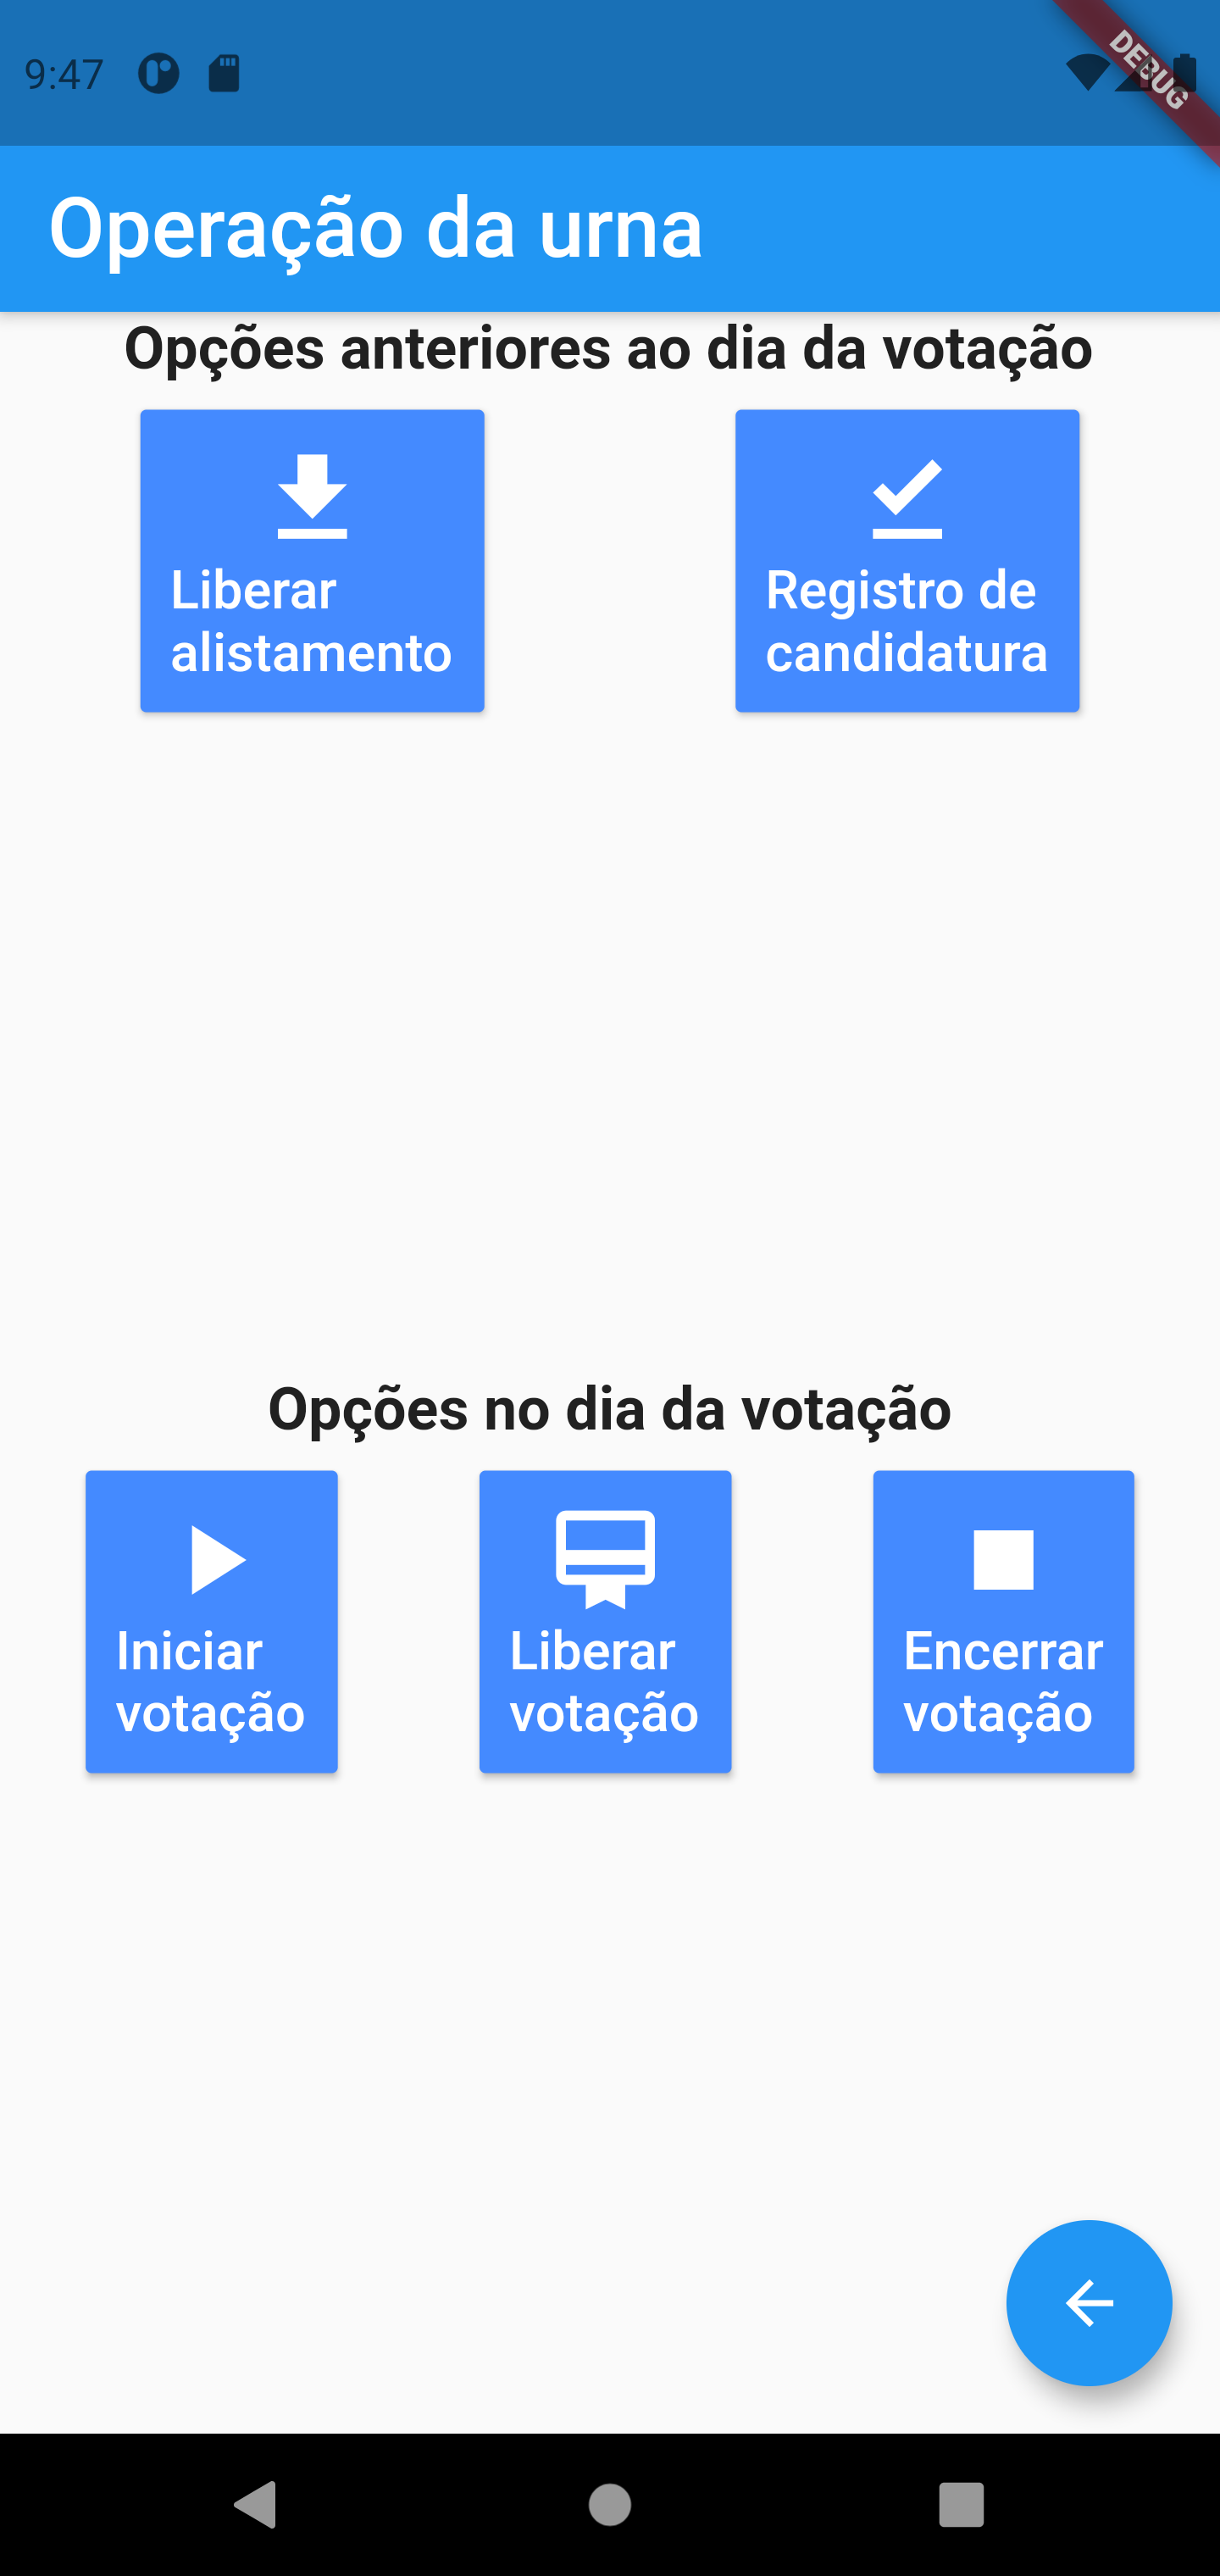
\includegraphics[width=0.5\textwidth]{imagens/wallet3}
	\caption{Módulo de operação das urnas}
	\label{fig:wallet_operador}
\end{figure}
\clearpage

\section{RDVE Coleta}

O RDVE Coleta\footnote{Código fonte disponível em \url{https://github.com/rammyres/rdve_coleta}} foi projetado em Python como um amalgama de dois projetos separados, o RDVE Coleta em si e o RDVE Urna.

\begin{figure}[h!]
	\centering
	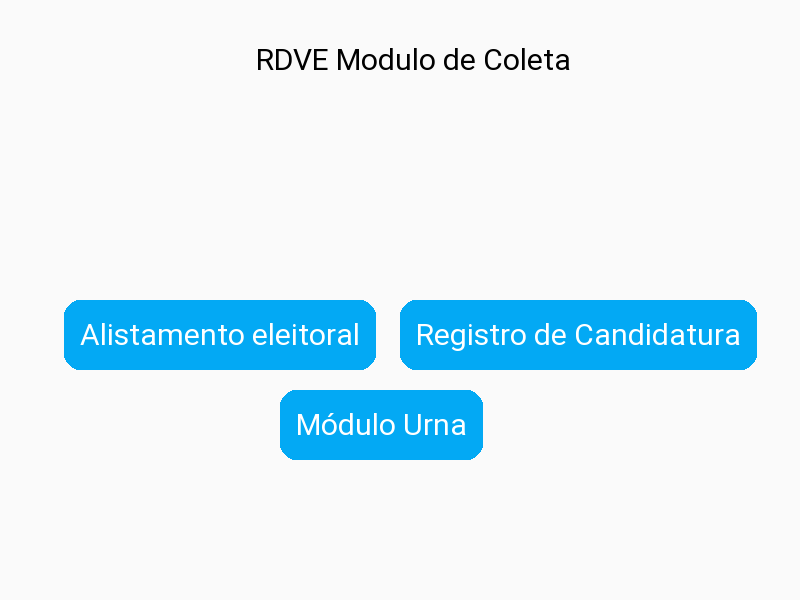
\includegraphics[width=0.8\textwidth]{imagens/coleta1}
	\caption{Sistema RDVE Coleta}
	\label{fig:coleta1}
\end{figure}

O RDVE Coleta registra eleitores e candidatos, bem como as requisições de votação, cédulas e os produtos de votação. Cada voto registrado na urna é procedido por uma aleatorização da lista de cédulas e somente ao final os votos, novamente embaralhados, tem seus \glspl{hash1} incluídos na \gls{merkle}, impedindo que se possa recuperar a ordem de votação por meios indiretos. 

\clearpage

\begin{figure}[!h]
	\centering
	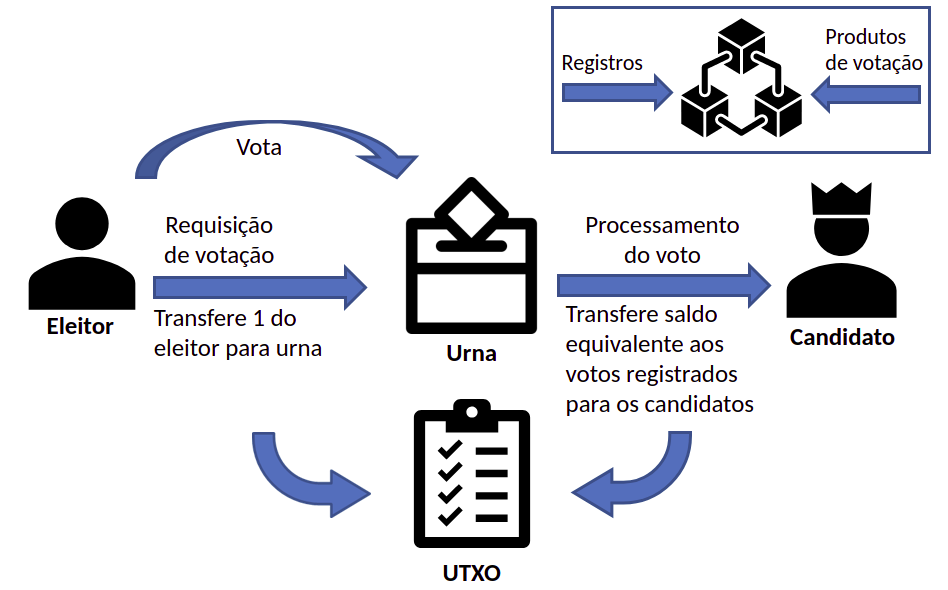
\includegraphics[width=0.9\textwidth]{imagens/fluxo_dados}
	\caption{Fluxo dos dados no sistema RDVE Coleta}
	\label{fig:fluxo_dados}
\end{figure}


\section{Resultados Obtidos}

A partir da execução dos aplicativos descritos foi possível realizar votações simuladas sem participações de terceiros, em decorrência da pandemia mundial de COVID-19.

Os registros representaram os dados inseridos e, em decorrência da forma de representação, mantiveram-se fidedignos e foi possível recuperar os estados registrados através da persistência dos objetos descritos acima como texto em formato \gls{json}. Os arquivos de registro e produtos de votação compreendiam blocos íntegros e todos os seus registros tinham entradas em sua \glspl{merkle} que podiam ter provas efetivamente produzíveis. 

Nas simulações não foi possível recuperar a ordem da votação ou cruzar o voto com o eleitor que o produziu. Em inspeção manual também foi possível verificar que o UTXO tinha saldos compatíveis com as transações existentes nos blocos de produtos de votação. 
\chapter{Discussão}
\chapter{Conclusão}
Muito se tem discutido sobre \gls{dlt} e, mais recentemente, \gls{bev}. A tecnologia empolga e traz consigo possibilidades grandes quanto ao futuro. As características inerentes a tecnologia trazem consigo grandes oportunidades e grandes desafios, entretanto a evolução tem sido significativa nos doze anos desde que o artigo de \citeonline{Nakamoto2008} foi publicado. 

O presente trabalho foi baseado em diversos trabalhos recentes sobre a tecnologia e suas implicações no sistema eleitoral e outros ramos do \gls{egov}. 

Com todas as considerações feitas, como a necessidade de mais pesquisas e ampliação dos mecanismos para testes, conforme expressado no capitulo anterior, nos parece que a proposta do projeto RDVE demonstrou ser capaz de produzir uma solução que atende aos requisitos da hipótese e viável para uso prático no mundo real, dado o amadurecimento necessário das ferramentas desenvolvidas. 

% ----------------------------------------------------------
% Capitulo com exemplos de comandos inseridos de arquivo externo 
% ----------------------------------------------------------

%\include{abntex2-modelo-inclCitaude-comandos}

% ---
% Finaliza a parte no bookmark do PDF
% para que se inicie o bookmark na raiz
% e adiciona espaço de parte no Sumário
% ---
\phantompart

% ---
% Conclusão
% ---

% ----------------------------------------------------------
% ELEMENTOS PÓS-TEXTUAIS
% ----------------------------------------------------------
\postextual

% ----------------------------------------------------------
% Referências bibliográficas
% ----------------------------------------------------------
\bibliography{postextuais/referencias}

% ----------------------------------------------------------
% Glossário
% ----------------------------------------------------------
%
% Consulte o manual da classe abntex2 para orientações sobre o glossário.
%

%\printglossaries

\glossary{postextuais/glossarios}
\printglossaries

% ----------------------------------------------------------
% Apêndices
% ----------------------------------------------------------

% ---
% Inicia os apêndices
% ---
\begin{apendicesenv}

% Imprime uma página indicando o início dos apêndices
% ↓ Remova o '%' para imprimir o inicio da parte dos apêndices
%\partapendices

% O que for incluido por aqui até o end serão os aprendices

\chapter{Fluxo de votação na Urna}

\begin{figure}[h!]
	\centering
	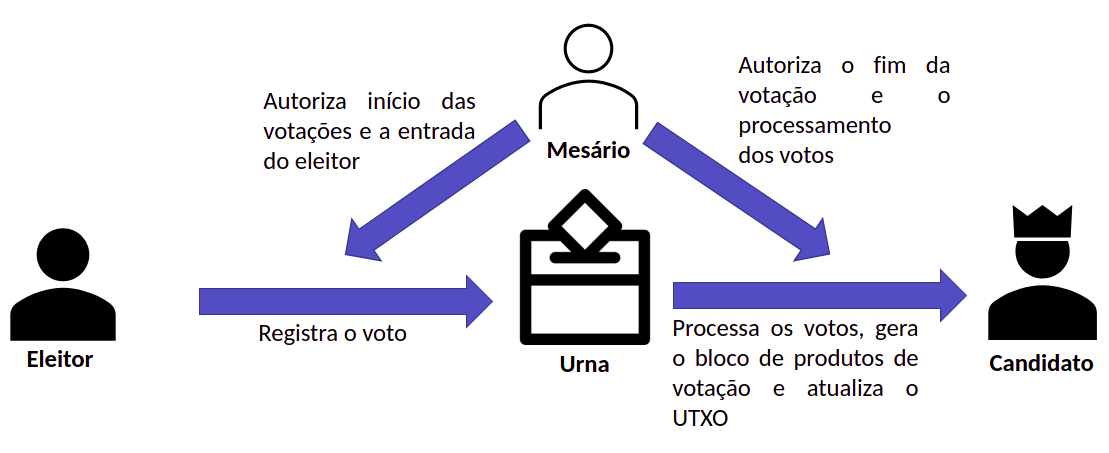
\includegraphics[width=0.9\textwidth]{imagens/fluxo_urna}
	\caption{Fluxo de controle da Urna}
	\label{fig:fluxo_urna}
\end{figure}
\chapter{Fluxo de geração de Bloco Produtos de Votação}

\begin{figure}[h!]
	\centering
	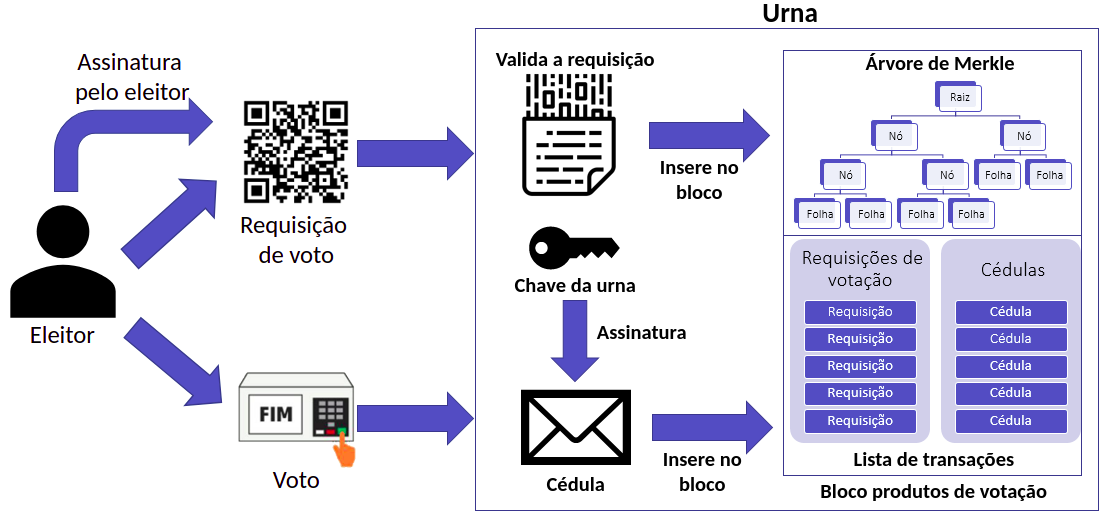
\includegraphics[width=\textwidth]{imagens/fluxo_voto}
	\caption{Fluxo do processo de geração do bloco Produtos de Votaçao}
	\label{fig:fluxo_voto}
\end{figure}

\end{apendicesenv}
\apendices
% ---


% ----------------------------------------------------------
% Anexos
% ----------------------------------------------------------

% ---
% Inicia os anexos
% ---
\begin{anexosenv}

% Imprime uma página indicando o início dos anexos
% ↓ Remova o '%' para imprimir o inicio da parte dos anexos
  %\partanexos
 
%O que for incluido por aqui até o end será considerado anexo

\end{anexosenv}

%---------------------------------------------------------------------
% INDICE REMISSIVO
%---------------------------------------------------------------------

\phantompart

\printindex


\end{document}
